\documentclass[10pt,english,a4paper]{article}
\usepackage[T1]{url}
\usepackage[utf8]{inputenc}
\usepackage[hidelinks]{hyperref} %colorlinks=true, linkcolor=blue!90!black
\usepackage{graphicx, varioref, babel, fancyvrb, listings, amsmath,amsthm, amssymb, enumerate, mathtools}
\usepackage{tikz}

\usepackage{pgfplots}
%%\usepackage{tikz-cd}

\usetikzlibrary{patterns}
\usetikzlibrary{arrows}
\usetikzlibrary{patterns}
\usetikzlibrary{shapes.misc}
\usetikzlibrary{arrows.meta} % requiers tikz v3.0 or newer
\tikzset{cross/.style={cross out, draw, 
         minimum size=2*(#1-\pgflinewidth), 
         inner sep=0pt, outer sep=0pt},
         cross/.default={3pt}}


\begin{document}

\begin{figure}
\centering
\begin{tikzpicture}[scale=0.85]
    \draw (-2.7, 0) -- (3.7, 0);
\draw (0, -1) -- (0, 4.7);
\draw[-{Latex[length=5mm, width=2mm]}] (0, 0) -- (0.923454, 2.53717) node[right] {$n$};
\draw[-{Latex[length=2mm, width=1mm]}] (1.485,0)  arc (0:70:1.485) node[midway, right] {$\theta$};
\draw (4.08455,2.4508) node[above] {$l_{t,\theta}$} -- (-2.02345, 4.67393);
\draw[dashed] (-2.81908,1.02606) -- (1.87939, -0.68404);
\draw[{Latex[length=2mm, width=1mm]}-{Latex[length=2mm, width=1mm]}] (-1.87939,0.68404) -- (-0.613911, 4.1609) node[midway, left] {$t$};

\end{tikzpicture}
    \caption{The parametrization $(t, \theta)$
of lines in the plane. (Figure 2.3).}
\end{figure}    

\begin{figure}
\centering
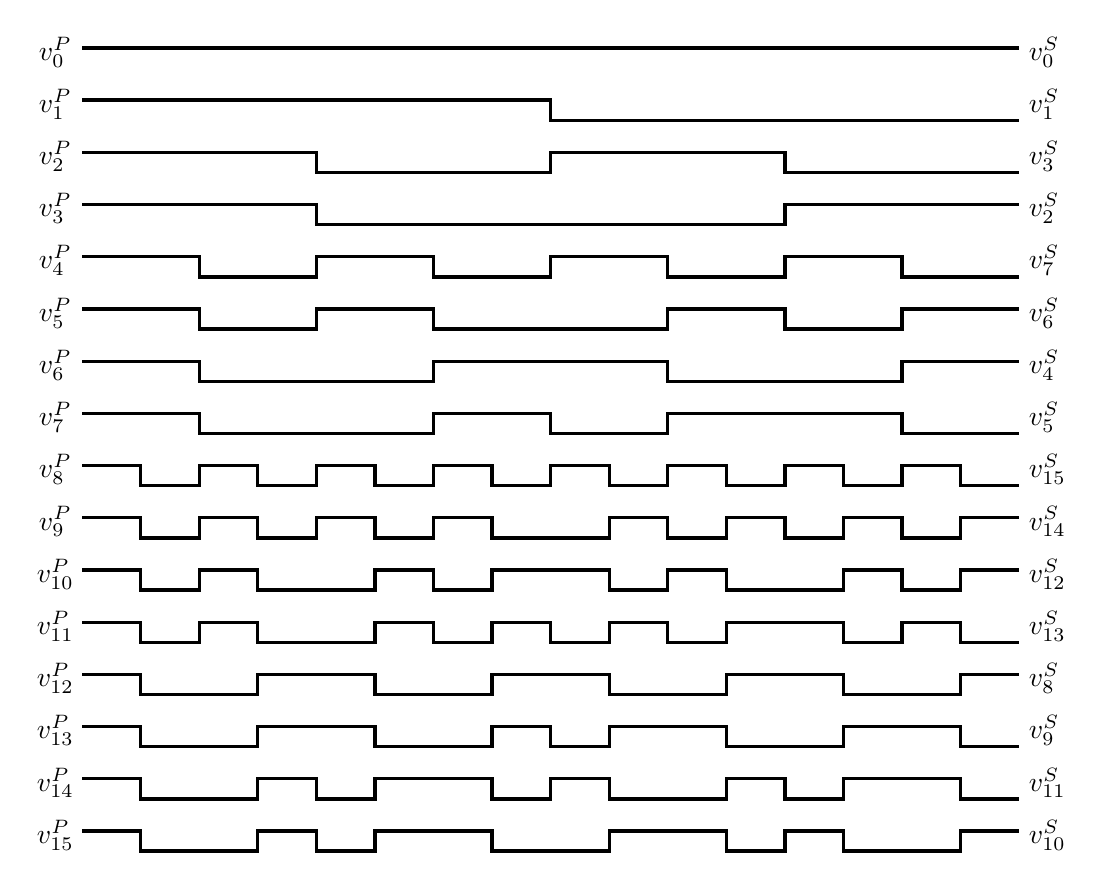
\begin{tikzpicture}[scale=0.85]
    \draw[very thick]  (0, 12) -- (0.875, 12) -- (13.125, 12) -- (13.125, 12)-- (13.125, 12) -- (14, 12);
        \draw (-0.4, 11.94) node {$v_{0}^{P}$};
        \draw (14, 11.94) node[right]  {$v_{0}^{S}$};
        \draw[very thick]  (0, 11.22) -- (0.875, 11.22) -- (7, 11.22) -- (7, 10.92) -- (13.125, 10.92) -- (13.125, 10.92)-- (13.125, 10.92) -- (14, 10.92);
        \draw (-0.4, 11.16) node {$v_{1}^{P}$};
        \draw (14, 11.16) node[right]  {$v_{1}^{S}$};
        \draw[very thick]  (0, 10.44) -- (0.875, 10.44) -- (3.5, 10.44) -- (3.5, 10.14) -- (7, 10.14) -- (7, 10.44) -- (10.5, 10.44) -- (10.5, 10.14) -- (13.125, 10.14) -- (13.125, 10.14)-- (13.125, 10.14) -- (14, 10.14);
        \draw (-0.4, 10.38) node {$v_{2}^{P}$};
        \draw (14, 10.38) node[right]  {$v_{3}^{S}$};
        \draw[very thick]  (0, 9.66) -- (0.875, 9.66) -- (3.5, 9.66) -- (3.5, 9.36) -- (10.5, 9.36) -- (10.5, 9.66) -- (13.125, 9.66) -- (13.125, 9.66)-- (13.125, 9.66) -- (14, 9.66);
        \draw (-0.4, 9.6) node {$v_{3}^{P}$};
        \draw (14, 9.6) node[right]  {$v_{2}^{S}$};
        \draw[very thick]  (0, 8.88) -- (0.875, 8.88) -- (1.75, 8.88) -- (1.75, 8.58) -- (3.5, 8.58) -- (3.5, 8.88) -- (5.25, 8.88) -- (5.25, 8.58) -- (7, 8.58) -- (7, 8.88) -- (8.75, 8.88) -- (8.75, 8.58) -- (10.5, 8.58) -- (10.5, 8.88) -- (12.25, 8.88) -- (12.25, 8.58) -- (13.125, 8.58) -- (13.125, 8.58)-- (13.125, 8.58) -- (14, 8.58);
        \draw (-0.4, 8.82) node {$v_{4}^{P}$};
        \draw (14, 8.82) node[right]  {$v_{7}^{S}$};
        \draw[very thick]  (0, 8.1) -- (0.875, 8.1) -- (1.75, 8.1) -- (1.75, 7.8) -- (3.5, 7.8) -- (3.5, 8.1) -- (5.25, 8.1) -- (5.25, 7.8) -- (8.75, 7.8) -- (8.75, 8.1) -- (10.5, 8.1) -- (10.5, 7.8) -- (12.25, 7.8) -- (12.25, 8.1) -- (13.125, 8.1) -- (13.125, 8.1)-- (13.125, 8.1) -- (14, 8.1);
        \draw (-0.4, 8.04) node {$v_{5}^{P}$};
        \draw (14, 8.04) node[right]  {$v_{6}^{S}$};
        \draw[very thick]  (0, 7.32) -- (0.875, 7.32) -- (1.75, 7.32) -- (1.75, 7.02) -- (5.25, 7.02) -- (5.25, 7.32) -- (8.75, 7.32) -- (8.75, 7.02) -- (12.25, 7.02) -- (12.25, 7.32) -- (13.125, 7.32) -- (13.125, 7.32)-- (13.125, 7.32) -- (14, 7.32);
        \draw (-0.4, 7.26) node {$v_{6}^{P}$};
        \draw (14, 7.26) node[right]  {$v_{4}^{S}$};
        \draw[very thick]  (0, 6.54) -- (0.875, 6.54) -- (1.75, 6.54) -- (1.75, 6.24) -- (5.25, 6.24) -- (5.25, 6.54) -- (7, 6.54) -- (7, 6.24) -- (8.75, 6.24) -- (8.75, 6.54) -- (12.25, 6.54) -- (12.25, 6.24) -- (13.125, 6.24) -- (13.125, 6.24)-- (13.125, 6.24) -- (14, 6.24);
        \draw (-0.4, 6.48) node {$v_{7}^{P}$};
        \draw (14, 6.48) node[right]  {$v_{5}^{S}$};
        \draw[very thick]  (0, 5.76) -- (0.875, 5.76) -- (0.875, 5.76) -- (0.875, 5.46) -- (1.75, 5.46) -- (1.75, 5.76) -- (2.625, 5.76) -- (2.625, 5.46) -- (3.5, 5.46) -- (3.5, 5.76) -- (4.375, 5.76) -- (4.375, 5.46) -- (5.25, 5.46) -- (5.25, 5.76) -- (6.125, 5.76) -- (6.125, 5.46) -- (7, 5.46) -- (7, 5.76) -- (7.875, 5.76) -- (7.875, 5.46) -- (8.75, 5.46) -- (8.75, 5.76) -- (9.625, 5.76) -- (9.625, 5.46) -- (10.5, 5.46) -- (10.5, 5.76) -- (11.375, 5.76) -- (11.375, 5.46) -- (12.25, 5.46) -- (12.25, 5.76) -- (13.125, 5.76) -- (13.125, 5.46)-- (13.125, 5.46) -- (14, 5.46);
        \draw (-0.4, 5.7) node {$v_{8}^{P}$};
        \draw (14, 5.7) node[right]  {$v_{15}^{S}$};
        \draw[very thick]  (0, 4.98) -- (0.875, 4.98) -- (0.875, 4.98) -- (0.875, 4.68) -- (1.75, 4.68) -- (1.75, 4.98) -- (2.625, 4.98) -- (2.625, 4.68) -- (3.5, 4.68) -- (3.5, 4.98) -- (4.375, 4.98) -- (4.375, 4.68) -- (5.25, 4.68) -- (5.25, 4.98) -- (6.125, 4.98) -- (6.125, 4.68) -- (7.875, 4.68) -- (7.875, 4.98) -- (8.75, 4.98) -- (8.75, 4.68) -- (9.625, 4.68) -- (9.625, 4.98) -- (10.5, 4.98) -- (10.5, 4.68) -- (11.375, 4.68) -- (11.375, 4.98) -- (12.25, 4.98) -- (12.25, 4.68) -- (13.125, 4.68) -- (13.125, 4.98)-- (13.125, 4.98) -- (14, 4.98);
        \draw (-0.4, 4.92) node {$v_{9}^{P}$};
        \draw (14, 4.92) node[right]  {$v_{14}^{S}$};
        \draw[very thick]  (0, 4.2) -- (0.875, 4.2) -- (0.875, 4.2) -- (0.875, 3.9) -- (1.75, 3.9) -- (1.75, 4.2) -- (2.625, 4.2) -- (2.625, 3.9) -- (4.375, 3.9) -- (4.375, 4.2) -- (5.25, 4.2) -- (5.25, 3.9) -- (6.125, 3.9) -- (6.125, 4.2) -- (7.875, 4.2) -- (7.875, 3.9) -- (8.75, 3.9) -- (8.75, 4.2) -- (9.625, 4.2) -- (9.625, 3.9) -- (11.375, 3.9) -- (11.375, 4.2) -- (12.25, 4.2) -- (12.25, 3.9) -- (13.125, 3.9) -- (13.125, 4.2)-- (13.125, 4.2) -- (14, 4.2);
        \draw (-0.4, 4.14) node {$v_{10}^{P}$};
        \draw (14, 4.14) node[right]  {$v_{12}^{S}$};
        \draw[very thick]  (0, 3.42) -- (0.875, 3.42) -- (0.875, 3.42) -- (0.875, 3.12) -- (1.75, 3.12) -- (1.75, 3.42) -- (2.625, 3.42) -- (2.625, 3.12) -- (4.375, 3.12) -- (4.375, 3.42) -- (5.25, 3.42) -- (5.25, 3.12) -- (6.125, 3.12) -- (6.125, 3.42) -- (7, 3.42) -- (7, 3.12) -- (7.875, 3.12) -- (7.875, 3.42) -- (8.75, 3.42) -- (8.75, 3.12) -- (9.625, 3.12) -- (9.625, 3.42) -- (11.375, 3.42) -- (11.375, 3.12) -- (12.25, 3.12) -- (12.25, 3.42) -- (13.125, 3.42) -- (13.125, 3.12)-- (13.125, 3.12) -- (14, 3.12);
        \draw (-0.4, 3.36) node {$v_{11}^{P}$};
        \draw (14, 3.36) node[right]  {$v_{13}^{S}$};
        \draw[very thick]  (0, 2.64) -- (0.875, 2.64) -- (0.875, 2.64) -- (0.875, 2.34) -- (2.625, 2.34) -- (2.625, 2.64) -- (4.375, 2.64) -- (4.375, 2.34) -- (6.125, 2.34) -- (6.125, 2.64) -- (7.875, 2.64) -- (7.875, 2.34) -- (9.625, 2.34) -- (9.625, 2.64) -- (11.375, 2.64) -- (11.375, 2.34) -- (13.125, 2.34) -- (13.125, 2.64)-- (13.125, 2.64) -- (14, 2.64);
        \draw (-0.4, 2.58) node {$v_{12}^{P}$};
        \draw (14, 2.58) node[right]  {$v_{8}^{S}$};
        \draw[very thick]  (0, 1.86) -- (0.875, 1.86) -- (0.875, 1.86) -- (0.875, 1.56) -- (2.625, 1.56) -- (2.625, 1.86) -- (4.375, 1.86) -- (4.375, 1.56) -- (6.125, 1.56) -- (6.125, 1.86) -- (7, 1.86) -- (7, 1.56) -- (7.875, 1.56) -- (7.875, 1.86) -- (9.625, 1.86) -- (9.625, 1.56) -- (11.375, 1.56) -- (11.375, 1.86) -- (13.125, 1.86) -- (13.125, 1.56)-- (13.125, 1.56) -- (14, 1.56);
        \draw (-0.4, 1.8) node {$v_{13}^{P}$};
        \draw (14, 1.8) node[right]  {$v_{9}^{S}$};
        \draw[very thick]  (0, 1.08) -- (0.875, 1.08) -- (0.875, 1.08) -- (0.875, 0.78) -- (2.625, 0.78) -- (2.625, 1.08) -- (3.5, 1.08) -- (3.5, 0.78) -- (4.375, 0.78) -- (4.375, 1.08) -- (6.125, 1.08) -- (6.125, 0.78) -- (7, 0.78) -- (7, 1.08) -- (7.875, 1.08) -- (7.875, 0.78) -- (9.625, 0.78) -- (9.625, 1.08) -- (10.5, 1.08) -- (10.5, 0.78) -- (11.375, 0.78) -- (11.375, 1.08) -- (13.125, 1.08) -- (13.125, 0.78)-- (13.125, 0.78) -- (14, 0.78);
        \draw (-0.4, 1.02) node {$v_{14}^{P}$};
        \draw (14, 1.02) node[right]  {$v_{11}^{S}$};
        \draw[very thick]  (0, 0.3) -- (0.875, 0.3) -- (0.875, 0.3) -- (0.875, 1.38778e-15) -- (2.625, 1.38778e-15) -- (2.625, 0.3) -- (3.5, 0.3) -- (3.5, 1.38778e-15) -- (4.375, 1.38778e-15) -- (4.375, 0.3) -- (6.125, 0.3) -- (6.125, 1.38778e-15) -- (7.875, 1.38778e-15) -- (7.875, 0.3) -- (9.625, 0.3) -- (9.625, 1.38778e-15) -- (10.5, 1.38778e-15) -- (10.5, 0.3) -- (11.375, 0.3) -- (11.375, 1.38778e-15) -- (13.125, 1.38778e-15) -- (13.125, 0.3)-- (13.125, 0.3) -- (14, 0.3);
        \draw (-0.4, 0.24) node {$v_{15}^{P}$};
        \draw (14, 0.24) node[right]  {$v_{10}^{S}$};
        
\end{tikzpicture}
    \caption{The 16 first Walsh functions 
with the Paley $(v_{n}^{P})$ or sequency $(v_{n}^{S})$ orderings.
(Figure 2.4).}
\end{figure}    


\begin{figure}
\begin{center}
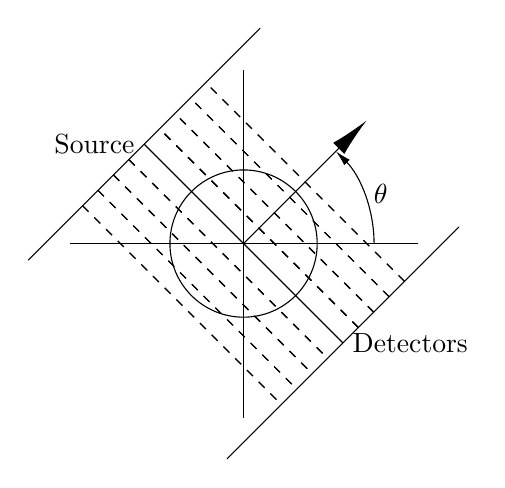
\begin{tikzpicture}[scale=0.85]
\draw (0,0) circle (1.1);
\draw (-2.6, 0) -- (2.6, 0);
\draw (0, -2.6) -- (0, 2.6);
\draw (0.247487,3.21734) -- (-3.21734, -0.247487);
\draw (-0.247487,-3.21734) -- (3.21734, 0.247487);
\draw[dashed] (-2.40416,0.565685) -- (0.565685, -2.40416);
\draw[dashed] (2.40416,-0.565685) -- (-0.565685, 2.40416);
\draw[dashed] (-2.17435,0.795495) -- (0.795495, -2.17435);
\draw[dashed] (2.17435,-0.795495) -- (-0.795495, 2.17435);
\draw[dashed] (-1.94454,1.0253) -- (1.0253, -1.94454);
\draw[dashed] (1.94454,-1.0253) -- (-1.0253, 1.94454);
\draw[dashed] (-1.71473,1.25511) -- (1.25511, -1.71473);
\draw[dashed] (1.71473,-1.25511) -- (-1.25511, 1.71473);
\draw (-1.48492,1.48492) -- (1.48492, -1.48492);
\draw[dashed] (1.71473,-1.25511) -- (-1.25511, 1.71473);
\draw[dashed] (-1.71473,1.25511) -- (1.25511, -1.71473);
\draw[dashed] (1.71473,-1.25511) -- (-1.25511, 1.71473);
\draw[dashed] (-1.94454,1.0253) -- (1.0253, -1.94454);
\draw[dashed] (1.94454,-1.0253) -- (-1.0253, 1.94454);
\draw[dashed] (-2.17435,0.795495) -- (0.795495, -2.17435);
\draw[dashed] (2.17435,-0.795495) -- (-0.795495, 2.17435);
\draw[dashed] (-2.40416,0.565685) -- (0.565685, -2.40416);
\draw[dashed] (2.40416,-0.565685) -- (-0.565685, 2.40416);
\draw[-{Latex[length=5mm, width=2mm]}] (0,0) -- (1.83848,1.83848);
\draw[-{Latex[length=2mm, width=1mm]}] (1.95,0)  arc (0:45:1.95) node[midway, right] {$\theta$};
\draw (1.48492,-1.48492)  node[right] {Detectors};
\draw (-1.48492,1.48492)  node[left] {Source};
\end{tikzpicture}
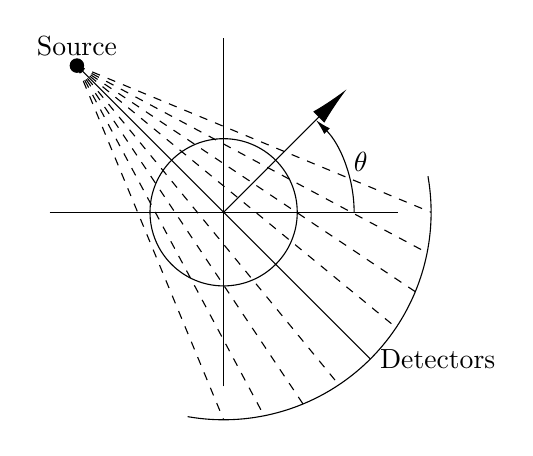
\begin{tikzpicture}[scale=0.85]
\draw (0,0) circle (1.1);
\draw (-2.6, 0) -- (2.6, 0);
\draw (0, -2.6) -- (0, 2.6);
\draw (3.0529,0.538309)  arc (10:-100:3.1) node[midway, right] {Detectors};
\filldraw[black] (-2.19203,2.19203)  circle (0.1) node[above] {Source};
\draw[dashed] (-2.19203,2.19203) -- (1.8982e-16, -3.1);
\draw[dashed] (-2.19203,2.19203) -- (0.60478, -3.04043);
\draw[dashed] (-2.19203,2.19203) -- (1.18632, -2.86403);
\draw[dashed] (-2.19203,2.19203) -- (1.72227, -2.57756);
\draw (-2.19203,2.19203) -- (2.19203, -2.19203);
\draw[dashed] (-2.19203,2.19203) -- (2.57756, -1.72227);
\draw[dashed] (-2.19203,2.19203) -- (2.86403, -1.18632);
\draw[dashed] (-2.19203,2.19203) -- (3.04043, -0.60478);
\draw[dashed] (-2.19203,2.19203) -- (3.1, 0);
\draw[-{Latex[length=5mm, width=2mm]}] (0,0) -- (1.83848,1.83848);
\draw[-{Latex[length=2mm, width=1mm]}] (1.95,0)  arc (0:45:1.95) node[midway, right] {$\theta$};
\end{tikzpicture}
\end{center}
\caption{
Typical geometries in X-ray CT. Left: Parallel beam. Right: Fan beam. (Figure 3.6)}

\end{figure}


\begin{figure}    
\centering
 \begin{tabular}{@{}c@{\hspace{0.05\linewidth}}c@{}}
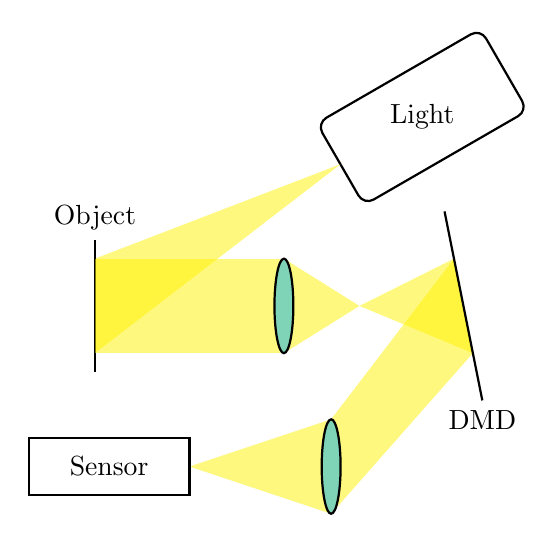
\begin{tikzpicture}[scale=1.2]
    \draw[thick, rounded corners, rotate around ={30:(1,0.5)}] (4,0) rectangle (6,1) node[midway] {Light};
    \fill[yellow, opacity=0.5] (1,0) -- (1,1) -- (3.6,2.0) --cycle;
    \draw[thick, rounded corners] (1,-0.2) -- (1,1.2) node[above] {Object};
    \fill[yellow, opacity=0.5] (1,0) rectangle (3,1);
    %\fill[yellow, opacity=0.5] (3,0) -- (5,0) --  (4.8,1) -- (3,1) --cycle;
    \fill[yellow, opacity=0.5] (3,0) -- (3.8, 0.5) -- (3,1) -- cycle; 
    \fill[yellow, opacity=0.5] (3.8, 0.5) -- (5,0) -- (4.8,1) -- cycle; 
    \fill[cyan, opacity=0.5] (3,0.5) ellipse (0.1 and 0.5);
    \draw[thick] (3,0.5) ellipse (0.1 and 0.5);
    \fill[yellow, opacity=0.5] (4.8,1) -- (3.5, -0.7)  --(3.5, -1.7) -- (5, 0) --cycle;
    \draw[thick] (4.7, 1.5) -- (5.1, -0.5) node[below] {DMD};
    \fill[yellow, opacity=0.5] (3.5, -0.7) -- (3.5, -1.7) -- (2, -1.2) -- cycle;
    \fill[cyan, opacity=0.5] (3.5,-1.2) ellipse (0.1 and 0.5); 
    \draw[thick] (3.5,-1.2) ellipse (0.1 and 0.5);
    \draw[thick] (0.3, -1.5) rectangle (2, -0.9) node[midway] {Sensor};
\end{tikzpicture}
&
    \centering
    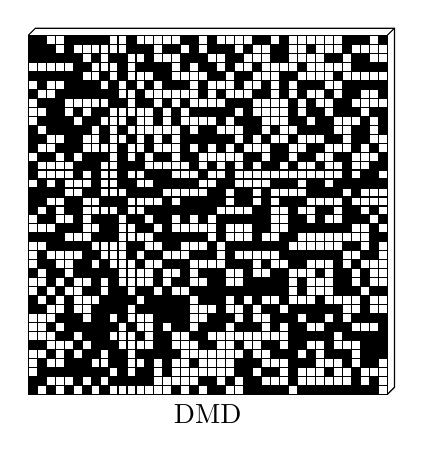
\begin{tikzpicture}[scale=0.57]
       \draw (0,0) rectangle (8,8);
\draw (0.2,0) -- (0.2, 8);
\draw (0,0.2) -- (8, 0.2);
\draw (0.4,0) -- (0.4, 8);
\draw (0,0.4) -- (8, 0.4);
\draw (0.6,0) -- (0.6, 8);
\draw (0,0.6) -- (8, 0.6);
\draw (0.8,0) -- (0.8, 8);
\draw (0,0.8) -- (8, 0.8);
\draw (1,0) -- (1, 8);
\draw (0,1) -- (8, 1);
\draw (1.2,0) -- (1.2, 8);
\draw (0,1.2) -- (8, 1.2);
\draw (1.4,0) -- (1.4, 8);
\draw (0,1.4) -- (8, 1.4);
\draw (1.6,0) -- (1.6, 8);
\draw (0,1.6) -- (8, 1.6);
\draw (1.8,0) -- (1.8, 8);
\draw (0,1.8) -- (8, 1.8);
\draw (2,0) -- (2, 8);
\draw (0,2) -- (8, 2);
\draw (2.2,0) -- (2.2, 8);
\draw (0,2.2) -- (8, 2.2);
\draw (2.4,0) -- (2.4, 8);
\draw (0,2.4) -- (8, 2.4);
\draw (2.6,0) -- (2.6, 8);
\draw (0,2.6) -- (8, 2.6);
\draw (2.8,0) -- (2.8, 8);
\draw (0,2.8) -- (8, 2.8);
\draw (3,0) -- (3, 8);
\draw (0,3) -- (8, 3);
\draw (3.2,0) -- (3.2, 8);
\draw (0,3.2) -- (8, 3.2);
\draw (3.4,0) -- (3.4, 8);
\draw (0,3.4) -- (8, 3.4);
\draw (3.6,0) -- (3.6, 8);
\draw (0,3.6) -- (8, 3.6);
\draw (3.8,0) -- (3.8, 8);
\draw (0,3.8) -- (8, 3.8);
\draw (4,0) -- (4, 8);
\draw (0,4) -- (8, 4);
\draw (4.2,0) -- (4.2, 8);
\draw (0,4.2) -- (8, 4.2);
\draw (4.4,0) -- (4.4, 8);
\draw (0,4.4) -- (8, 4.4);
\draw (4.6,0) -- (4.6, 8);
\draw (0,4.6) -- (8, 4.6);
\draw (4.8,0) -- (4.8, 8);
\draw (0,4.8) -- (8, 4.8);
\draw (5,0) -- (5, 8);
\draw (0,5) -- (8, 5);
\draw (5.2,0) -- (5.2, 8);
\draw (0,5.2) -- (8, 5.2);
\draw (5.4,0) -- (5.4, 8);
\draw (0,5.4) -- (8, 5.4);
\draw (5.6,0) -- (5.6, 8);
\draw (0,5.6) -- (8, 5.6);
\draw (5.8,0) -- (5.8, 8);
\draw (0,5.8) -- (8, 5.8);
\draw (6,0) -- (6, 8);
\draw (0,6) -- (8, 6);
\draw (6.2,0) -- (6.2, 8);
\draw (0,6.2) -- (8, 6.2);
\draw (6.4,0) -- (6.4, 8);
\draw (0,6.4) -- (8, 6.4);
\draw (6.6,0) -- (6.6, 8);
\draw (0,6.6) -- (8, 6.6);
\draw (6.8,0) -- (6.8, 8);
\draw (0,6.8) -- (8, 6.8);
\draw (7,0) -- (7, 8);
\draw (0,7) -- (8, 7);
\draw (7.2,0) -- (7.2, 8);
\draw (0,7.2) -- (8, 7.2);
\draw (7.4,0) -- (7.4, 8);
\draw (0,7.4) -- (8, 7.4);
\draw (7.6,0) -- (7.6, 8);
\draw (0,7.6) -- (8, 7.6);
\draw (7.8,0) -- (7.8, 8);
\draw (0,7.8) -- (8, 7.8);
\filldraw[black] (0, 0) rectangle (0.2, 0.2);
\filldraw[black] (0, 0.2) rectangle (0.2, 0.4);
\filldraw[black] (0, 1) rectangle (0.2, 1.2);
\filldraw[black] (0, 1.8) rectangle (0.2, 2);
\filldraw[black] (0, 2) rectangle (0.2, 2.2);
\filldraw[black] (0, 2.6) rectangle (0.2, 2.8);
\filldraw[black] (0, 3.4) rectangle (0.2, 3.6);
\filldraw[black] (0, 4) rectangle (0.2, 4.2);
\filldraw[black] (0, 4.2) rectangle (0.2, 4.4);
\filldraw[black] (0, 4.4) rectangle (0.2, 4.6);
\filldraw[black] (0, 4.8) rectangle (0.2, 5);
\filldraw[black] (0, 5) rectangle (0.2, 5.2);
\filldraw[black] (0, 5.4) rectangle (0.2, 5.6);
\filldraw[black] (0, 5.6) rectangle (0.2, 5.8);
\filldraw[black] (0, 5.8) rectangle (0.2, 6);
\filldraw[black] (0, 6.6) rectangle (0.2, 6.8);
\filldraw[black] (0, 7) rectangle (0.2, 7.2);
\filldraw[black] (0, 7.4) rectangle (0.2, 7.6);
\filldraw[black] (0, 7.6) rectangle (0.2, 7.8);
\filldraw[black] (0, 7.8) rectangle (0.2, 8);
\filldraw[black] (0.2, 0.2) rectangle (0.4, 0.4);
\filldraw[black] (0.2, 0.4) rectangle (0.4, 0.6);
\filldraw[black] (0.2, 0.6) rectangle (0.4, 0.8);
\filldraw[black] (0.2, 1) rectangle (0.4, 1.2);
\filldraw[black] (0.2, 1.8) rectangle (0.4, 2);
\filldraw[black] (0.2, 2.2) rectangle (0.4, 2.4);
\filldraw[black] (0.2, 2.8) rectangle (0.4, 3);
\filldraw[black] (0.2, 3) rectangle (0.4, 3.2);
\filldraw[black] (0.2, 3.4) rectangle (0.4, 3.6);
\filldraw[black] (0.2, 3.8) rectangle (0.4, 4);
\filldraw[black] (0.2, 4.2) rectangle (0.4, 4.4);
\filldraw[black] (0.2, 4.4) rectangle (0.4, 4.6);
\filldraw[black] (0.2, 4.6) rectangle (0.4, 4.8);
\filldraw[black] (0.2, 5.2) rectangle (0.4, 5.4);
\filldraw[black] (0.2, 5.6) rectangle (0.4, 5.8);
\filldraw[black] (0.2, 6) rectangle (0.4, 6.2);
\filldraw[black] (0.2, 6.4) rectangle (0.4, 6.6);
\filldraw[black] (0.2, 6.8) rectangle (0.4, 7);
\filldraw[black] (0.2, 7) rectangle (0.4, 7.2);
\filldraw[black] (0.2, 7.4) rectangle (0.4, 7.6);
\filldraw[black] (0.2, 7.6) rectangle (0.4, 7.8);
\filldraw[black] (0.2, 7.8) rectangle (0.4, 8);
\filldraw[black] (0.4, 0) rectangle (0.6, 0.2);
\filldraw[black] (0.4, 0.4) rectangle (0.6, 0.6);
\filldraw[black] (0.4, 0.8) rectangle (0.6, 1);
\filldraw[black] (0.4, 1.4) rectangle (0.6, 1.6);
\filldraw[black] (0.4, 2) rectangle (0.6, 2.2);
\filldraw[black] (0.4, 2.4) rectangle (0.6, 2.6);
\filldraw[black] (0.4, 2.6) rectangle (0.6, 2.8);
\filldraw[black] (0.4, 2.8) rectangle (0.6, 3);
\filldraw[black] (0.4, 3.2) rectangle (0.6, 3.4);
\filldraw[black] (0.4, 3.4) rectangle (0.6, 3.6);
\filldraw[black] (0.4, 3.8) rectangle (0.6, 4);
\filldraw[black] (0.4, 4) rectangle (0.6, 4.2);
\filldraw[black] (0.4, 4.4) rectangle (0.6, 4.6);
\filldraw[black] (0.4, 5.2) rectangle (0.6, 5.4);
\filldraw[black] (0.4, 5.8) rectangle (0.6, 6);
\filldraw[black] (0.4, 6) rectangle (0.6, 6.2);
\filldraw[black] (0.4, 6.2) rectangle (0.6, 6.4);
\filldraw[black] (0.4, 6.4) rectangle (0.6, 6.6);
\filldraw[black] (0.4, 7) rectangle (0.6, 7.2);
\filldraw[black] (0.4, 7.4) rectangle (0.6, 7.6);
\filldraw[black] (0.4, 7.6) rectangle (0.6, 7.8);
\filldraw[black] (0.6, 0.4) rectangle (0.8, 0.6);
\filldraw[black] (0.6, 1.2) rectangle (0.8, 1.4);
\filldraw[black] (0.6, 1.6) rectangle (0.8, 1.8);
\filldraw[black] (0.6, 2.2) rectangle (0.8, 2.4);
\filldraw[black] (0.6, 2.6) rectangle (0.8, 2.8);
\filldraw[black] (0.6, 3.2) rectangle (0.8, 3.4);
\filldraw[black] (0.6, 3.4) rectangle (0.8, 3.6);
\filldraw[black] (0.6, 3.6) rectangle (0.8, 3.8);
\filldraw[black] (0.6, 4.4) rectangle (0.8, 4.6);
\filldraw[black] (0.6, 4.6) rectangle (0.8, 4.8);
\filldraw[black] (0.6, 5.4) rectangle (0.8, 5.6);
\filldraw[black] (0.6, 5.8) rectangle (0.8, 6);
\filldraw[black] (0.6, 6) rectangle (0.8, 6.2);
\filldraw[black] (0.6, 6.2) rectangle (0.8, 6.4);
\filldraw[black] (0.6, 6.4) rectangle (0.8, 6.6);
\filldraw[black] (0.6, 6.6) rectangle (0.8, 6.8);
\filldraw[black] (0.6, 7) rectangle (0.8, 7.2);
\filldraw[black] (0.6, 7.4) rectangle (0.8, 7.6);
\filldraw[black] (0.8, 0) rectangle (1, 0.2);
\filldraw[black] (0.8, 0.4) rectangle (1, 0.6);
\filldraw[black] (0.8, 0.6) rectangle (1, 0.8);
\filldraw[black] (0.8, 0.8) rectangle (1, 1);
\filldraw[black] (0.8, 1.2) rectangle (1, 1.4);
\filldraw[black] (0.8, 1.4) rectangle (1, 1.6);
\filldraw[black] (0.8, 1.6) rectangle (1, 1.8);
\filldraw[black] (0.8, 1.8) rectangle (1, 2);
\filldraw[black] (0.8, 2) rectangle (1, 2.2);
\filldraw[black] (0.8, 2.4) rectangle (1, 2.6);
\filldraw[black] (0.8, 3.2) rectangle (1, 3.4);
\filldraw[black] (0.8, 3.6) rectangle (1, 3.8);
\filldraw[black] (0.8, 4) rectangle (1, 4.2);
\filldraw[black] (0.8, 4.2) rectangle (1, 4.4);
\filldraw[black] (0.8, 5.2) rectangle (1, 5.4);
\filldraw[black] (0.8, 5.4) rectangle (1, 5.6);
\filldraw[black] (0.8, 5.6) rectangle (1, 5.8);
\filldraw[black] (0.8, 5.8) rectangle (1, 6);
\filldraw[black] (0.8, 6) rectangle (1, 6.2);
\filldraw[black] (0.8, 6.6) rectangle (1, 6.8);
\filldraw[black] (0.8, 6.8) rectangle (1, 7);
\filldraw[black] (0.8, 7) rectangle (1, 7.2);
\filldraw[black] (0.8, 7.4) rectangle (1, 7.6);
\filldraw[black] (0.8, 7.6) rectangle (1, 7.8);
\filldraw[black] (0.8, 7.8) rectangle (1, 8);
\filldraw[black] (1, 0.2) rectangle (1.2, 0.4);
\filldraw[black] (1, 0.4) rectangle (1.2, 0.6);
\filldraw[black] (1, 0.6) rectangle (1.2, 0.8);
\filldraw[black] (1, 1) rectangle (1.2, 1.2);
\filldraw[black] (1, 1.4) rectangle (1.2, 1.6);
\filldraw[black] (1, 1.6) rectangle (1.2, 1.8);
\filldraw[black] (1, 2.6) rectangle (1.2, 2.8);
\filldraw[black] (1, 2.8) rectangle (1.2, 3);
\filldraw[black] (1, 3.2) rectangle (1.2, 3.4);
\filldraw[black] (1, 3.6) rectangle (1.2, 3.8);
\filldraw[black] (1, 3.8) rectangle (1.2, 4);
\filldraw[black] (1, 4) rectangle (1.2, 4.2);
\filldraw[black] (1, 4.2) rectangle (1.2, 4.4);
\filldraw[black] (1, 4.8) rectangle (1.2, 5);
\filldraw[black] (1, 5) rectangle (1.2, 5.2);
\filldraw[black] (1, 5.4) rectangle (1.2, 5.6);
\filldraw[black] (1, 5.6) rectangle (1.2, 5.8);
\filldraw[black] (1, 5.8) rectangle (1.2, 6);
\filldraw[black] (1, 6.2) rectangle (1.2, 6.4);
\filldraw[black] (1, 6.6) rectangle (1.2, 6.8);
\filldraw[black] (1, 6.8) rectangle (1.2, 7);
\filldraw[black] (1, 7) rectangle (1.2, 7.2);
\filldraw[black] (1, 7.2) rectangle (1.2, 7.4);
\filldraw[black] (1, 7.4) rectangle (1.2, 7.6);
\filldraw[black] (1, 7.8) rectangle (1.2, 8);
\filldraw[black] (1.2, 0) rectangle (1.4, 0.2);
\filldraw[black] (1.2, 0.4) rectangle (1.4, 0.6);
\filldraw[black] (1.2, 0.6) rectangle (1.4, 0.8);
\filldraw[black] (1.2, 0.8) rectangle (1.4, 1);
\filldraw[black] (1.2, 1.2) rectangle (1.4, 1.4);
\filldraw[black] (1.2, 1.4) rectangle (1.4, 1.6);
\filldraw[black] (1.2, 2.2) rectangle (1.4, 2.4);
\filldraw[black] (1.2, 2.6) rectangle (1.4, 2.8);
\filldraw[black] (1.2, 2.8) rectangle (1.4, 3);
\filldraw[black] (1.2, 3) rectangle (1.4, 3.2);
\filldraw[black] (1.2, 3.2) rectangle (1.4, 3.4);
\filldraw[black] (1.2, 4.4) rectangle (1.4, 4.6);
\filldraw[black] (1.2, 5) rectangle (1.4, 5.2);
\filldraw[black] (1.2, 5.2) rectangle (1.4, 5.4);
\filldraw[black] (1.2, 5.8) rectangle (1.4, 6);
\filldraw[black] (1.2, 6) rectangle (1.4, 6.2);
\filldraw[black] (1.2, 6.6) rectangle (1.4, 6.8);
\filldraw[black] (1.2, 6.8) rectangle (1.4, 7);
\filldraw[black] (1.2, 7.2) rectangle (1.4, 7.4);
\filldraw[black] (1.2, 7.8) rectangle (1.4, 8);
\filldraw[black] (1.4, 0.2) rectangle (1.6, 0.4);
\filldraw[black] (1.4, 0.4) rectangle (1.6, 0.6);
\filldraw[black] (1.4, 0.8) rectangle (1.6, 1);
\filldraw[black] (1.4, 1) rectangle (1.6, 1.2);
\filldraw[black] (1.4, 1.2) rectangle (1.6, 1.4);
\filldraw[black] (1.4, 1.4) rectangle (1.6, 1.6);
\filldraw[black] (1.4, 1.6) rectangle (1.6, 1.8);
\filldraw[black] (1.4, 1.8) rectangle (1.6, 2);
\filldraw[black] (1.4, 2.2) rectangle (1.6, 2.4);
\filldraw[black] (1.4, 2.4) rectangle (1.6, 2.6);
\filldraw[black] (1.4, 2.6) rectangle (1.6, 2.8);
\filldraw[black] (1.4, 3) rectangle (1.6, 3.2);
\filldraw[black] (1.4, 3.4) rectangle (1.6, 3.6);
\filldraw[black] (1.4, 3.8) rectangle (1.6, 4);
\filldraw[black] (1.4, 4.4) rectangle (1.6, 4.6);
\filldraw[black] (1.4, 4.6) rectangle (1.6, 4.8);
\filldraw[black] (1.4, 4.8) rectangle (1.6, 5);
\filldraw[black] (1.4, 5) rectangle (1.6, 5.2);
\filldraw[black] (1.4, 5.2) rectangle (1.6, 5.4);
\filldraw[black] (1.4, 6) rectangle (1.6, 6.2);
\filldraw[black] (1.4, 6.2) rectangle (1.6, 6.4);
\filldraw[black] (1.4, 6.6) rectangle (1.6, 6.8);
\filldraw[black] (1.4, 6.8) rectangle (1.6, 7);
\filldraw[black] (1.4, 7.4) rectangle (1.6, 7.6);
\filldraw[black] (1.4, 7.8) rectangle (1.6, 8);
\filldraw[black] (1.6, 0) rectangle (1.8, 0.2);
\filldraw[black] (1.6, 0.4) rectangle (1.8, 0.6);
\filldraw[black] (1.6, 1) rectangle (1.8, 1.2);
\filldraw[black] (1.6, 1.2) rectangle (1.8, 1.4);
\filldraw[black] (1.6, 1.4) rectangle (1.8, 1.6);
\filldraw[black] (1.6, 1.6) rectangle (1.8, 1.8);
\filldraw[black] (1.6, 1.8) rectangle (1.8, 2);
\filldraw[black] (1.6, 2) rectangle (1.8, 2.2);
\filldraw[black] (1.6, 2.6) rectangle (1.8, 2.8);
\filldraw[black] (1.6, 2.8) rectangle (1.8, 3);
\filldraw[black] (1.6, 3.4) rectangle (1.8, 3.6);
\filldraw[black] (1.6, 3.6) rectangle (1.8, 3.8);
\filldraw[black] (1.6, 3.8) rectangle (1.8, 4);
\filldraw[black] (1.6, 4.2) rectangle (1.8, 4.4);
\filldraw[black] (1.6, 5.2) rectangle (1.8, 5.4);
\filldraw[black] (1.6, 5.6) rectangle (1.8, 5.8);
\filldraw[black] (1.6, 5.8) rectangle (1.8, 6);
\filldraw[black] (1.6, 6.2) rectangle (1.8, 6.4);
\filldraw[black] (1.6, 6.6) rectangle (1.8, 6.8);
\filldraw[black] (1.6, 7) rectangle (1.8, 7.2);
\filldraw[black] (1.6, 7.8) rectangle (1.8, 8);
\filldraw[black] (1.8, 0.2) rectangle (2, 0.4);
\filldraw[black] (1.8, 0.6) rectangle (2, 0.8);
\filldraw[black] (1.8, 0.8) rectangle (2, 1);
\filldraw[black] (1.8, 1) rectangle (2, 1.2);
\filldraw[black] (1.8, 1.4) rectangle (2, 1.6);
\filldraw[black] (1.8, 1.8) rectangle (2, 2);
\filldraw[black] (1.8, 2) rectangle (2, 2.2);
\filldraw[black] (1.8, 2.2) rectangle (2, 2.4);
\filldraw[black] (1.8, 2.4) rectangle (2, 2.6);
\filldraw[black] (1.8, 2.6) rectangle (2, 2.8);
\filldraw[black] (1.8, 3.4) rectangle (2, 3.6);
\filldraw[black] (1.8, 3.6) rectangle (2, 3.8);
\filldraw[black] (1.8, 3.8) rectangle (2, 4);
\filldraw[black] (1.8, 4.2) rectangle (2, 4.4);
\filldraw[black] (1.8, 6.4) rectangle (2, 6.6);
\filldraw[black] (1.8, 6.6) rectangle (2, 6.8);
\filldraw[black] (1.8, 6.8) rectangle (2, 7);
\filldraw[black] (1.8, 7.4) rectangle (2, 7.6);
\filldraw[black] (2, 0.2) rectangle (2.2, 0.4);
\filldraw[black] (2, 0.4) rectangle (2.2, 0.6);
\filldraw[black] (2, 0.6) rectangle (2.2, 0.8);
\filldraw[black] (2, 0.8) rectangle (2.2, 1);
\filldraw[black] (2, 1.6) rectangle (2.2, 1.8);
\filldraw[black] (2, 1.8) rectangle (2.2, 2);
\filldraw[black] (2, 2) rectangle (2.2, 2.2);
\filldraw[black] (2, 2.2) rectangle (2.2, 2.4);
\filldraw[black] (2, 4) rectangle (2.2, 4.2);
\filldraw[black] (2, 4.2) rectangle (2.2, 4.4);
\filldraw[black] (2, 4.6) rectangle (2.2, 4.8);
\filldraw[black] (2, 4.8) rectangle (2.2, 5);
\filldraw[black] (2, 5) rectangle (2.2, 5.2);
\filldraw[black] (2, 5.2) rectangle (2.2, 5.4);
\filldraw[black] (2, 5.4) rectangle (2.2, 5.6);
\filldraw[black] (2, 5.8) rectangle (2.2, 6);
\filldraw[black] (2, 6.4) rectangle (2.2, 6.6);
\filldraw[black] (2, 7) rectangle (2.2, 7.2);
\filldraw[black] (2, 7.2) rectangle (2.2, 7.4);
\filldraw[black] (2, 7.4) rectangle (2.2, 7.6);
\filldraw[black] (2.2, 0.2) rectangle (2.4, 0.4);
\filldraw[black] (2.2, 1.4) rectangle (2.4, 1.6);
\filldraw[black] (2.2, 2) rectangle (2.4, 2.2);
\filldraw[black] (2.2, 3) rectangle (2.4, 3.2);
\filldraw[black] (2.2, 3.2) rectangle (2.4, 3.4);
\filldraw[black] (2.2, 3.8) rectangle (2.4, 4);
\filldraw[black] (2.2, 4.4) rectangle (2.4, 4.6);
\filldraw[black] (2.2, 4.6) rectangle (2.4, 4.8);
\filldraw[black] (2.2, 5) rectangle (2.4, 5.2);
\filldraw[black] (2.2, 5.6) rectangle (2.4, 5.8);
\filldraw[black] (2.2, 6) rectangle (2.4, 6.2);
\filldraw[black] (2.2, 6.8) rectangle (2.4, 7);
\filldraw[black] (2.2, 7.6) rectangle (2.4, 7.8);
\filldraw[black] (2.2, 7.8) rectangle (2.4, 8);
\filldraw[black] (2.4, 0.2) rectangle (2.6, 0.4);
\filldraw[black] (2.4, 0.4) rectangle (2.6, 0.6);
\filldraw[black] (2.4, 0.8) rectangle (2.6, 1);
\filldraw[black] (2.4, 1.2) rectangle (2.6, 1.4);
\filldraw[black] (2.4, 1.8) rectangle (2.6, 2);
\filldraw[black] (2.4, 2.2) rectangle (2.6, 2.4);
\filldraw[black] (2.4, 2.8) rectangle (2.6, 3);
\filldraw[black] (2.4, 3.2) rectangle (2.6, 3.4);
\filldraw[black] (2.4, 3.6) rectangle (2.6, 3.8);
\filldraw[black] (2.4, 3.8) rectangle (2.6, 4);
\filldraw[black] (2.4, 4.4) rectangle (2.6, 4.6);
\filldraw[black] (2.4, 5) rectangle (2.6, 5.2);
\filldraw[black] (2.4, 5.2) rectangle (2.6, 5.4);
\filldraw[black] (2.4, 6.4) rectangle (2.6, 6.6);
\filldraw[black] (2.4, 6.6) rectangle (2.6, 6.8);
\filldraw[black] (2.4, 7.2) rectangle (2.6, 7.4);
\filldraw[black] (2.4, 7.6) rectangle (2.6, 7.8);
\filldraw[black] (2.6, 0.2) rectangle (2.8, 0.4);
\filldraw[black] (2.6, 0.4) rectangle (2.8, 0.6);
\filldraw[black] (2.6, 0.6) rectangle (2.8, 0.8);
\filldraw[black] (2.6, 0.8) rectangle (2.8, 1);
\filldraw[black] (2.6, 1.8) rectangle (2.8, 2);
\filldraw[black] (2.6, 2) rectangle (2.8, 2.2);
\filldraw[black] (2.6, 2.2) rectangle (2.8, 2.4);
\filldraw[black] (2.6, 3) rectangle (2.8, 3.2);
\filldraw[black] (2.6, 3.6) rectangle (2.8, 3.8);
\filldraw[black] (2.6, 4) rectangle (2.8, 4.2);
\filldraw[black] (2.6, 4.4) rectangle (2.8, 4.6);
\filldraw[black] (2.6, 4.8) rectangle (2.8, 5);
\filldraw[black] (2.6, 5.4) rectangle (2.8, 5.6);
\filldraw[black] (2.6, 5.6) rectangle (2.8, 5.8);
\filldraw[black] (2.6, 6.4) rectangle (2.8, 6.6);
\filldraw[black] (2.6, 6.8) rectangle (2.8, 7);
\filldraw[black] (2.6, 7.2) rectangle (2.8, 7.4);
\filldraw[black] (2.6, 7.4) rectangle (2.8, 7.6);
\filldraw[black] (2.6, 7.6) rectangle (2.8, 7.8);
\filldraw[black] (2.8, 0.8) rectangle (3, 1);
\filldraw[black] (2.8, 1) rectangle (3, 1.2);
\filldraw[black] (2.8, 1.2) rectangle (3, 1.4);
\filldraw[black] (2.8, 1.4) rectangle (3, 1.6);
\filldraw[black] (2.8, 1.6) rectangle (3, 1.8);
\filldraw[black] (2.8, 1.8) rectangle (3, 2);
\filldraw[black] (2.8, 2) rectangle (3, 2.2);
\filldraw[black] (2.8, 2.4) rectangle (3, 2.6);
\filldraw[black] (2.8, 2.6) rectangle (3, 2.8);
\filldraw[black] (2.8, 3) rectangle (3, 3.2);
\filldraw[black] (2.8, 3.4) rectangle (3, 3.6);
\filldraw[black] (2.8, 3.8) rectangle (3, 4);
\filldraw[black] (2.8, 4) rectangle (3, 4.2);
\filldraw[black] (2.8, 4.4) rectangle (3, 4.6);
\filldraw[black] (2.8, 4.6) rectangle (3, 4.8);
\filldraw[black] (2.8, 4.8) rectangle (3, 5);
\filldraw[black] (2.8, 5.2) rectangle (3, 5.4);
\filldraw[black] (2.8, 6) rectangle (3, 6.2);
\filldraw[black] (2.8, 6.2) rectangle (3, 6.4);
\filldraw[black] (2.8, 7) rectangle (3, 7.2);
\filldraw[black] (2.8, 7.2) rectangle (3, 7.4);
\filldraw[black] (3, 0.4) rectangle (3.2, 0.6);
\filldraw[black] (3, 0.6) rectangle (3.2, 0.8);
\filldraw[black] (3, 0.8) rectangle (3.2, 1);
\filldraw[black] (3, 1) rectangle (3.2, 1.2);
\filldraw[black] (3, 1.2) rectangle (3.2, 1.4);
\filldraw[black] (3, 1.6) rectangle (3.2, 1.8);
\filldraw[black] (3, 1.8) rectangle (3.2, 2);
\filldraw[black] (3, 2) rectangle (3.2, 2.2);
\filldraw[black] (3, 2.2) rectangle (3.2, 2.4);
\filldraw[black] (3, 2.8) rectangle (3.2, 3);
\filldraw[black] (3, 3.2) rectangle (3.2, 3.4);
\filldraw[black] (3, 3.4) rectangle (3.2, 3.6);
\filldraw[black] (3, 3.6) rectangle (3.2, 3.8);
\filldraw[black] (3, 3.8) rectangle (3.2, 4);
\filldraw[black] (3, 4) rectangle (3.2, 4.2);
\filldraw[black] (3, 4.2) rectangle (3.2, 4.4);
\filldraw[black] (3, 4.6) rectangle (3.2, 4.8);
\filldraw[black] (3, 4.8) rectangle (3.2, 5);
\filldraw[black] (3, 5.2) rectangle (3.2, 5.4);
\filldraw[black] (3, 5.6) rectangle (3.2, 5.8);
\filldraw[black] (3, 6.4) rectangle (3.2, 6.6);
\filldraw[black] (3, 6.8) rectangle (3.2, 7);
\filldraw[black] (3, 7) rectangle (3.2, 7.2);
\filldraw[black] (3, 7.2) rectangle (3.2, 7.4);
\filldraw[black] (3, 7.6) rectangle (3.2, 7.8);
\filldraw[black] (3.2, 0) rectangle (3.4, 0.2);
\filldraw[black] (3.2, 0.8) rectangle (3.4, 1);
\filldraw[black] (3.2, 1.4) rectangle (3.4, 1.6);
\filldraw[black] (3.2, 1.6) rectangle (3.4, 1.8);
\filldraw[black] (3.2, 1.8) rectangle (3.4, 2);
\filldraw[black] (3.2, 2) rectangle (3.4, 2.2);
\filldraw[black] (3.2, 2.4) rectangle (3.4, 2.6);
\filldraw[black] (3.2, 2.8) rectangle (3.4, 3);
\filldraw[black] (3.2, 3.2) rectangle (3.4, 3.4);
\filldraw[black] (3.2, 3.4) rectangle (3.4, 3.6);
\filldraw[black] (3.2, 4) rectangle (3.4, 4.2);
\filldraw[black] (3.2, 4.6) rectangle (3.4, 4.8);
\filldraw[black] (3.2, 6) rectangle (3.4, 6.2);
\filldraw[black] (3.2, 6.2) rectangle (3.4, 6.4);
\filldraw[black] (3.2, 6.8) rectangle (3.4, 7);
\filldraw[black] (3.2, 7.6) rectangle (3.4, 7.8);
\filldraw[black] (3.4, 1.4) rectangle (3.6, 1.6);
\filldraw[black] (3.4, 1.6) rectangle (3.6, 1.8);
\filldraw[black] (3.4, 1.8) rectangle (3.6, 2);
\filldraw[black] (3.4, 2) rectangle (3.6, 2.2);
\filldraw[black] (3.4, 2.4) rectangle (3.6, 2.6);
\filldraw[black] (3.4, 2.6) rectangle (3.6, 2.8);
\filldraw[black] (3.4, 2.8) rectangle (3.6, 3);
\filldraw[black] (3.4, 3.4) rectangle (3.6, 3.6);
\filldraw[black] (3.4, 3.8) rectangle (3.6, 4);
\filldraw[black] (3.4, 4) rectangle (3.6, 4.2);
\filldraw[black] (3.4, 4.2) rectangle (3.6, 4.4);
\filldraw[black] (3.4, 4.6) rectangle (3.6, 4.8);
\filldraw[black] (3.4, 5.2) rectangle (3.6, 5.4);
\filldraw[black] (3.4, 5.4) rectangle (3.6, 5.6);
\filldraw[black] (3.4, 5.6) rectangle (3.6, 5.8);
\filldraw[black] (3.4, 5.8) rectangle (3.6, 6);
\filldraw[black] (3.4, 6.4) rectangle (3.6, 6.6);
\filldraw[black] (3.4, 6.8) rectangle (3.6, 7);
\filldraw[black] (3.4, 7.2) rectangle (3.6, 7.4);
\filldraw[black] (3.4, 7.4) rectangle (3.6, 7.6);
\filldraw[black] (3.4, 7.8) rectangle (3.6, 8);
\filldraw[black] (3.6, 0) rectangle (3.8, 0.2);
\filldraw[black] (3.6, 0.6) rectangle (3.8, 0.8);
\filldraw[black] (3.6, 1.2) rectangle (3.8, 1.4);
\filldraw[black] (3.6, 2.2) rectangle (3.8, 2.4);
\filldraw[black] (3.6, 3) rectangle (3.8, 3.2);
\filldraw[black] (3.6, 3.4) rectangle (3.8, 3.6);
\filldraw[black] (3.6, 4) rectangle (3.8, 4.2);
\filldraw[black] (3.6, 4.2) rectangle (3.8, 4.4);
\filldraw[black] (3.6, 4.6) rectangle (3.8, 4.8);
\filldraw[black] (3.6, 5) rectangle (3.8, 5.2);
\filldraw[black] (3.6, 5.2) rectangle (3.8, 5.4);
\filldraw[black] (3.6, 5.6) rectangle (3.8, 5.8);
\filldraw[black] (3.6, 6.2) rectangle (3.8, 6.4);
\filldraw[black] (3.6, 7.4) rectangle (3.8, 7.6);
\filldraw[black] (3.6, 7.6) rectangle (3.8, 7.8);
\filldraw[black] (3.6, 7.8) rectangle (3.8, 8);
\filldraw[black] (3.8, 0.2) rectangle (4, 0.4);
\filldraw[black] (3.8, 1) rectangle (4, 1.2);
\filldraw[black] (3.8, 1.2) rectangle (4, 1.4);
\filldraw[black] (3.8, 1.4) rectangle (4, 1.6);
\filldraw[black] (3.8, 2) rectangle (4, 2.2);
\filldraw[black] (3.8, 2.2) rectangle (4, 2.4);
\filldraw[black] (3.8, 2.6) rectangle (4, 2.8);
\filldraw[black] (3.8, 3) rectangle (4, 3.2);
\filldraw[black] (3.8, 3.4) rectangle (4, 3.6);
\filldraw[black] (3.8, 3.8) rectangle (4, 4);
\filldraw[black] (3.8, 4) rectangle (4, 4.2);
\filldraw[black] (3.8, 4.2) rectangle (4, 4.4);
\filldraw[black] (3.8, 4.8) rectangle (4, 5);
\filldraw[black] (3.8, 5.4) rectangle (4, 5.6);
\filldraw[black] (3.8, 5.6) rectangle (4, 5.8);
\filldraw[black] (3.8, 5.8) rectangle (4, 6);
\filldraw[black] (3.8, 6.2) rectangle (4, 6.4);
\filldraw[black] (3.8, 6.6) rectangle (4, 6.8);
\filldraw[black] (3.8, 6.8) rectangle (4, 7);
\filldraw[black] (3.8, 7.2) rectangle (4, 7.4);
\filldraw[black] (3.8, 7.4) rectangle (4, 7.6);
\filldraw[black] (4, 0) rectangle (4.2, 0.2);
\filldraw[black] (4, 0.2) rectangle (4.2, 0.4);
\filldraw[black] (4, 1) rectangle (4.2, 1.2);
\filldraw[black] (4, 1.4) rectangle (4.2, 1.6);
\filldraw[black] (4, 1.6) rectangle (4.2, 1.8);
\filldraw[black] (4, 2) rectangle (4.2, 2.2);
\filldraw[black] (4, 2.2) rectangle (4.2, 2.4);
\filldraw[black] (4, 2.4) rectangle (4.2, 2.6);
\filldraw[black] (4, 2.6) rectangle (4.2, 2.8);
\filldraw[black] (4, 3) rectangle (4.2, 3.2);
\filldraw[black] (4, 3.2) rectangle (4.2, 3.4);
\filldraw[black] (4, 4) rectangle (4.2, 4.2);
\filldraw[black] (4, 4.2) rectangle (4.2, 4.4);
\filldraw[black] (4, 4.4) rectangle (4.2, 4.6);
\filldraw[black] (4, 5) rectangle (4.2, 5.2);
\filldraw[black] (4, 5.6) rectangle (4.2, 5.8);
\filldraw[black] (4, 5.8) rectangle (4.2, 6);
\filldraw[black] (4, 6.2) rectangle (4.2, 6.4);
\filldraw[black] (4, 7) rectangle (4.2, 7.2);
\filldraw[black] (4, 7.2) rectangle (4.2, 7.4);
\filldraw[black] (4, 7.6) rectangle (4.2, 7.8);
\filldraw[black] (4, 7.8) rectangle (4.2, 8);
\filldraw[black] (4.2, 0) rectangle (4.4, 0.2);
\filldraw[black] (4.2, 1.4) rectangle (4.4, 1.6);
\filldraw[black] (4.2, 1.6) rectangle (4.4, 1.8);
\filldraw[black] (4.2, 1.8) rectangle (4.4, 2);
\filldraw[black] (4.2, 2) rectangle (4.4, 2.2);
\filldraw[black] (4.2, 2.2) rectangle (4.4, 2.4);
\filldraw[black] (4.2, 2.4) rectangle (4.4, 2.6);
\filldraw[black] (4.2, 2.6) rectangle (4.4, 2.8);
\filldraw[black] (4.2, 3.4) rectangle (4.4, 3.6);
\filldraw[black] (4.2, 3.6) rectangle (4.4, 3.8);
\filldraw[black] (4.2, 3.8) rectangle (4.4, 4);
\filldraw[black] (4.2, 4.2) rectangle (4.4, 4.4);
\filldraw[black] (4.2, 4.4) rectangle (4.4, 4.6);
\filldraw[black] (4.2, 4.6) rectangle (4.4, 4.8);
\filldraw[black] (4.2, 5.4) rectangle (4.4, 5.6);
\filldraw[black] (4.2, 5.6) rectangle (4.4, 5.8);
\filldraw[black] (4.2, 6) rectangle (4.4, 6.2);
\filldraw[black] (4.2, 6.2) rectangle (4.4, 6.4);
\filldraw[black] (4.2, 6.6) rectangle (4.4, 6.8);
\filldraw[black] (4.2, 7) rectangle (4.4, 7.2);
\filldraw[black] (4.2, 7.6) rectangle (4.4, 7.8);
\filldraw[black] (4.4, 0.2) rectangle (4.6, 0.4);
\filldraw[black] (4.4, 1.6) rectangle (4.6, 1.8);
\filldraw[black] (4.4, 2.2) rectangle (4.6, 2.4);
\filldraw[black] (4.4, 2.8) rectangle (4.6, 3);
\filldraw[black] (4.4, 3) rectangle (4.6, 3.2);
\filldraw[black] (4.4, 3.2) rectangle (4.6, 3.4);
\filldraw[black] (4.4, 3.8) rectangle (4.6, 4);
\filldraw[black] (4.4, 4.6) rectangle (4.6, 4.8);
\filldraw[black] (4.4, 4.8) rectangle (4.6, 5);
\filldraw[black] (4.4, 5) rectangle (4.6, 5.2);
\filldraw[black] (4.4, 5.6) rectangle (4.6, 5.8);
\filldraw[black] (4.4, 6.2) rectangle (4.6, 6.4);
\filldraw[black] (4.4, 6.4) rectangle (4.6, 6.6);
\filldraw[black] (4.4, 7.2) rectangle (4.6, 7.4);
\filldraw[black] (4.4, 7.4) rectangle (4.6, 7.6);
\filldraw[black] (4.4, 7.6) rectangle (4.6, 7.8);
\filldraw[black] (4.6, 0.4) rectangle (4.8, 0.6);
\filldraw[black] (4.6, 0.6) rectangle (4.8, 0.8);
\filldraw[black] (4.6, 1) rectangle (4.8, 1.2);
\filldraw[black] (4.6, 1.4) rectangle (4.8, 1.6);
\filldraw[black] (4.6, 2) rectangle (4.8, 2.2);
\filldraw[black] (4.6, 2.2) rectangle (4.8, 2.4);
\filldraw[black] (4.6, 2.8) rectangle (4.8, 3);
\filldraw[black] (4.6, 3.2) rectangle (4.8, 3.4);
\filldraw[black] (4.6, 3.8) rectangle (4.8, 4);
\filldraw[black] (4.6, 4.2) rectangle (4.8, 4.4);
\filldraw[black] (4.6, 4.4) rectangle (4.8, 4.6);
\filldraw[black] (4.6, 5.4) rectangle (4.8, 5.6);
\filldraw[black] (4.6, 6) rectangle (4.8, 6.2);
\filldraw[black] (4.6, 6.4) rectangle (4.8, 6.6);
\filldraw[black] (4.6, 6.8) rectangle (4.8, 7);
\filldraw[black] (4.6, 7) rectangle (4.8, 7.2);
\filldraw[black] (4.6, 7.4) rectangle (4.8, 7.6);
\filldraw[black] (4.8, 0) rectangle (5, 0.2);
\filldraw[black] (4.8, 0.2) rectangle (5, 0.4);
\filldraw[black] (4.8, 0.4) rectangle (5, 0.6);
\filldraw[black] (4.8, 0.6) rectangle (5, 0.8);
\filldraw[black] (4.8, 0.8) rectangle (5, 1);
\filldraw[black] (4.8, 1.4) rectangle (5, 1.6);
\filldraw[black] (4.8, 1.6) rectangle (5, 1.8);
\filldraw[black] (4.8, 1.8) rectangle (5, 2);
\filldraw[black] (4.8, 2.2) rectangle (5, 2.4);
\filldraw[black] (4.8, 2.4) rectangle (5, 2.6);
\filldraw[black] (4.8, 2.6) rectangle (5, 2.8);
\filldraw[black] (4.8, 2.8) rectangle (5, 3);
\filldraw[black] (4.8, 3.2) rectangle (5, 3.4);
\filldraw[black] (4.8, 3.8) rectangle (5, 4);
\filldraw[black] (4.8, 4.2) rectangle (5, 4.4);
\filldraw[black] (4.8, 4.4) rectangle (5, 4.6);
\filldraw[black] (4.8, 5) rectangle (5, 5.2);
\filldraw[black] (4.8, 5.2) rectangle (5, 5.4);
\filldraw[black] (4.8, 5.6) rectangle (5, 5.8);
\filldraw[black] (4.8, 5.8) rectangle (5, 6);
\filldraw[black] (4.8, 6) rectangle (5, 6.2);
\filldraw[black] (4.8, 6.2) rectangle (5, 6.4);
\filldraw[black] (4.8, 6.4) rectangle (5, 6.6);
\filldraw[black] (4.8, 7) rectangle (5, 7.2);
\filldraw[black] (4.8, 7.6) rectangle (5, 7.8);
\filldraw[black] (5, 0) rectangle (5.2, 0.2);
\filldraw[black] (5, 0.2) rectangle (5.2, 0.4);
\filldraw[black] (5, 0.6) rectangle (5.2, 0.8);
\filldraw[black] (5, 1.4) rectangle (5.2, 1.6);
\filldraw[black] (5, 2) rectangle (5.2, 2.2);
\filldraw[black] (5, 2.2) rectangle (5.2, 2.4);
\filldraw[black] (5, 2.4) rectangle (5.2, 2.6);
\filldraw[black] (5, 3.2) rectangle (5.2, 3.4);
\filldraw[black] (5, 3.4) rectangle (5.2, 3.6);
\filldraw[black] (5, 3.6) rectangle (5.2, 3.8);
\filldraw[black] (5, 3.8) rectangle (5.2, 4);
\filldraw[black] (5, 4) rectangle (5.2, 4.2);
\filldraw[black] (5, 5.2) rectangle (5.2, 5.4);
\filldraw[black] (5, 5.8) rectangle (5.2, 6);
\filldraw[black] (5, 6) rectangle (5.2, 6.2);
\filldraw[black] (5, 6.6) rectangle (5.2, 6.8);
\filldraw[black] (5, 7.2) rectangle (5.2, 7.4);
\filldraw[black] (5, 7.8) rectangle (5.2, 8);
\filldraw[black] (5.2, 0) rectangle (5.4, 0.2);
\filldraw[black] (5.2, 0.4) rectangle (5.4, 0.6);
\filldraw[black] (5.2, 1) rectangle (5.4, 1.2);
\filldraw[black] (5.2, 1.8) rectangle (5.4, 2);
\filldraw[black] (5.2, 2.2) rectangle (5.4, 2.4);
\filldraw[black] (5.2, 2.4) rectangle (5.4, 2.6);
\filldraw[black] (5.2, 2.8) rectangle (5.4, 3);
\filldraw[black] (5.2, 3.2) rectangle (5.4, 3.4);
\filldraw[black] (5.2, 3.6) rectangle (5.4, 3.8);
\filldraw[black] (5.2, 3.8) rectangle (5.4, 4);
\filldraw[black] (5.2, 4) rectangle (5.4, 4.2);
\filldraw[black] (5.2, 4.2) rectangle (5.4, 4.4);
\filldraw[black] (5.2, 4.4) rectangle (5.4, 4.6);
\filldraw[black] (5.2, 5) rectangle (5.4, 5.2);
\filldraw[black] (5.2, 5.6) rectangle (5.4, 5.8);
\filldraw[black] (5.2, 6.6) rectangle (5.4, 6.8);
\filldraw[black] (5.2, 6.8) rectangle (5.4, 7);
\filldraw[black] (5.2, 7.8) rectangle (5.4, 8);
\filldraw[black] (5.4, 0) rectangle (5.6, 0.2);
\filldraw[black] (5.4, 0.4) rectangle (5.6, 0.6);
\filldraw[black] (5.4, 0.8) rectangle (5.6, 1);
\filldraw[black] (5.4, 1) rectangle (5.6, 1.2);
\filldraw[black] (5.4, 1.4) rectangle (5.6, 1.6);
\filldraw[black] (5.4, 1.6) rectangle (5.6, 1.8);
\filldraw[black] (5.4, 1.8) rectangle (5.6, 2);
\filldraw[black] (5.4, 2.2) rectangle (5.6, 2.4);
\filldraw[black] (5.4, 2.4) rectangle (5.6, 2.6);
\filldraw[black] (5.4, 2.6) rectangle (5.6, 2.8);
\filldraw[black] (5.4, 3.2) rectangle (5.6, 3.4);
\filldraw[black] (5.4, 4.6) rectangle (5.6, 4.8);
\filldraw[black] (5.4, 5) rectangle (5.6, 5.2);
\filldraw[black] (5.4, 5.2) rectangle (5.6, 5.4);
\filldraw[black] (5.4, 5.4) rectangle (5.6, 5.6);
\filldraw[black] (5.4, 5.8) rectangle (5.6, 6);
\filldraw[black] (5.4, 7.4) rectangle (5.6, 7.6);
\filldraw[black] (5.4, 7.6) rectangle (5.6, 7.8);
\filldraw[black] (5.6, 0) rectangle (5.8, 0.2);
\filldraw[black] (5.6, 0.8) rectangle (5.8, 1);
\filldraw[black] (5.6, 1.6) rectangle (5.8, 1.8);
\filldraw[black] (5.6, 2) rectangle (5.8, 2.2);
\filldraw[black] (5.6, 2.2) rectangle (5.8, 2.4);
\filldraw[black] (5.6, 2.4) rectangle (5.8, 2.6);
\filldraw[black] (5.6, 2.6) rectangle (5.8, 2.8);
\filldraw[black] (5.6, 3) rectangle (5.8, 3.2);
\filldraw[black] (5.6, 3.2) rectangle (5.8, 3.4);
\filldraw[black] (5.6, 3.4) rectangle (5.8, 3.6);
\filldraw[black] (5.6, 4.2) rectangle (5.8, 4.4);
\filldraw[black] (5.6, 4.6) rectangle (5.8, 4.8);
\filldraw[black] (5.6, 5.2) rectangle (5.8, 5.4);
\filldraw[black] (5.6, 5.4) rectangle (5.8, 5.6);
\filldraw[black] (5.6, 6.6) rectangle (5.8, 6.8);
\filldraw[black] (5.6, 6.8) rectangle (5.8, 7);
\filldraw[black] (5.6, 7) rectangle (5.8, 7.2);
\filldraw[black] (5.6, 7.4) rectangle (5.8, 7.6);
\filldraw[black] (5.6, 7.6) rectangle (5.8, 7.8);
\filldraw[black] (5.6, 7.8) rectangle (5.8, 8);
\filldraw[black] (5.8, 0.2) rectangle (6, 0.4);
\filldraw[black] (5.8, 0.4) rectangle (6, 0.6);
\filldraw[black] (5.8, 0.6) rectangle (6, 0.8);
\filldraw[black] (5.8, 0.8) rectangle (6, 1);
\filldraw[black] (5.8, 1) rectangle (6, 1.2);
\filldraw[black] (5.8, 1.2) rectangle (6, 1.4);
\filldraw[black] (5.8, 1.4) rectangle (6, 1.6);
\filldraw[black] (5.8, 1.6) rectangle (6, 1.8);
\filldraw[black] (5.8, 1.8) rectangle (6, 2);
\filldraw[black] (5.8, 2.8) rectangle (6, 3);
\filldraw[black] (5.8, 3) rectangle (6, 3.2);
\filldraw[black] (5.8, 3.4) rectangle (6, 3.6);
\filldraw[black] (5.8, 3.6) rectangle (6, 3.8);
\filldraw[black] (5.8, 3.8) rectangle (6, 4);
\filldraw[black] (5.8, 4) rectangle (6, 4.2);
\filldraw[black] (5.8, 4.2) rectangle (6, 4.4);
\filldraw[black] (5.8, 4.6) rectangle (6, 4.8);
\filldraw[black] (5.8, 5) rectangle (6, 5.2);
\filldraw[black] (5.8, 5.6) rectangle (6, 5.8);
\filldraw[black] (5.8, 6) rectangle (6, 6.2);
\filldraw[black] (5.8, 6.2) rectangle (6, 6.4);
\filldraw[black] (5.8, 6.4) rectangle (6, 6.6);
\filldraw[black] (5.8, 7) rectangle (6, 7.2);
\filldraw[black] (6, 0) rectangle (6.2, 0.2);
\filldraw[black] (6, 0.6) rectangle (6.2, 0.8);
\filldraw[black] (6, 1) rectangle (6.2, 1.2);
\filldraw[black] (6, 1.2) rectangle (6.2, 1.4);
\filldraw[black] (6, 1.4) rectangle (6.2, 1.6);
\filldraw[black] (6, 1.8) rectangle (6.2, 2);
\filldraw[black] (6, 2.2) rectangle (6.2, 2.4);
\filldraw[black] (6, 2.4) rectangle (6.2, 2.6);
\filldraw[black] (6, 2.8) rectangle (6.2, 3);
\filldraw[black] (6, 3) rectangle (6.2, 3.2);
\filldraw[black] (6, 3.6) rectangle (6.2, 3.8);
\filldraw[black] (6, 3.8) rectangle (6.2, 4);
\filldraw[black] (6, 4.2) rectangle (6.2, 4.4);
\filldraw[black] (6, 5.2) rectangle (6.2, 5.4);
\filldraw[black] (6, 5.8) rectangle (6.2, 6);
\filldraw[black] (6, 6) rectangle (6.2, 6.2);
\filldraw[black] (6, 6.6) rectangle (6.2, 6.8);
\filldraw[black] (6, 6.8) rectangle (6.2, 7);
\filldraw[black] (6, 7.2) rectangle (6.2, 7.4);
\filldraw[black] (6.2, 0) rectangle (6.4, 0.2);
\filldraw[black] (6.2, 0.6) rectangle (6.4, 0.8);
\filldraw[black] (6.2, 0.8) rectangle (6.4, 1);
\filldraw[black] (6.2, 1.2) rectangle (6.4, 1.4);
\filldraw[black] (6.2, 1.6) rectangle (6.4, 1.8);
\filldraw[black] (6.2, 1.8) rectangle (6.4, 2);
\filldraw[black] (6.2, 3) rectangle (6.4, 3.2);
\filldraw[black] (6.2, 3.6) rectangle (6.4, 3.8);
\filldraw[black] (6.2, 4.4) rectangle (6.4, 4.6);
\filldraw[black] (6.2, 4.6) rectangle (6.4, 4.8);
\filldraw[black] (6.2, 5.2) rectangle (6.4, 5.4);
\filldraw[black] (6.2, 5.4) rectangle (6.4, 5.6);
\filldraw[black] (6.2, 5.8) rectangle (6.4, 6);
\filldraw[black] (6.2, 6.2) rectangle (6.4, 6.4);
\filldraw[black] (6.2, 6.4) rectangle (6.4, 6.6);
\filldraw[black] (6.2, 6.8) rectangle (6.4, 7);
\filldraw[black] (6.2, 7.6) rectangle (6.4, 7.8);
\filldraw[black] (6.4, 0) rectangle (6.6, 0.2);
\filldraw[black] (6.4, 1.2) rectangle (6.6, 1.4);
\filldraw[black] (6.4, 1.6) rectangle (6.6, 1.8);
\filldraw[black] (6.4, 1.8) rectangle (6.6, 2);
\filldraw[black] (6.4, 2) rectangle (6.6, 2.2);
\filldraw[black] (6.4, 2.6) rectangle (6.6, 2.8);
\filldraw[black] (6.4, 3) rectangle (6.6, 3.2);
\filldraw[black] (6.4, 3.6) rectangle (6.6, 3.8);
\filldraw[black] (6.4, 3.8) rectangle (6.6, 4);
\filldraw[black] (6.4, 4) rectangle (6.6, 4.2);
\filldraw[black] (6.4, 4.4) rectangle (6.6, 4.6);
\filldraw[black] (6.4, 4.6) rectangle (6.6, 4.8);
\filldraw[black] (6.4, 5) rectangle (6.6, 5.2);
\filldraw[black] (6.4, 5.4) rectangle (6.6, 5.6);
\filldraw[black] (6.4, 5.8) rectangle (6.6, 6);
\filldraw[black] (6.4, 6) rectangle (6.6, 6.2);
\filldraw[black] (6.4, 6.2) rectangle (6.6, 6.4);
\filldraw[black] (6.4, 6.8) rectangle (6.6, 7);
\filldraw[black] (6.6, 0) rectangle (6.8, 0.2);
\filldraw[black] (6.6, 0.4) rectangle (6.8, 0.6);
\filldraw[black] (6.6, 0.8) rectangle (6.8, 1);
\filldraw[black] (6.6, 1) rectangle (6.8, 1.2);
\filldraw[black] (6.6, 1.2) rectangle (6.8, 1.4);
\filldraw[black] (6.6, 1.4) rectangle (6.8, 1.6);
\filldraw[black] (6.6, 1.8) rectangle (6.8, 2);
\filldraw[black] (6.6, 3) rectangle (6.8, 3.2);
\filldraw[black] (6.6, 3.6) rectangle (6.8, 3.8);
\filldraw[black] (6.6, 4) rectangle (6.8, 4.2);
\filldraw[black] (6.6, 4.4) rectangle (6.8, 4.6);
\filldraw[black] (6.6, 5.6) rectangle (6.8, 5.8);
\filldraw[black] (6.6, 5.8) rectangle (6.8, 6);
\filldraw[black] (6.6, 6) rectangle (6.8, 6.2);
\filldraw[black] (6.6, 6.6) rectangle (6.8, 6.8);
\filldraw[black] (6.6, 7.4) rectangle (6.8, 7.6);
\filldraw[black] (6.8, 0) rectangle (7, 0.2);
\filldraw[black] (6.8, 0.8) rectangle (7, 1);
\filldraw[black] (6.8, 1.4) rectangle (7, 1.6);
\filldraw[black] (6.8, 1.6) rectangle (7, 1.8);
\filldraw[black] (6.8, 1.8) rectangle (7, 2);
\filldraw[black] (6.8, 2.2) rectangle (7, 2.4);
\filldraw[black] (6.8, 2.4) rectangle (7, 2.6);
\filldraw[black] (6.8, 2.6) rectangle (7, 2.8);
\filldraw[black] (6.8, 2.8) rectangle (7, 3);
\filldraw[black] (6.8, 3) rectangle (7, 3.2);
\filldraw[black] (6.8, 3.6) rectangle (7, 3.8);
\filldraw[black] (6.8, 4.4) rectangle (7, 4.6);
\filldraw[black] (6.8, 4.6) rectangle (7, 4.8);
\filldraw[black] (6.8, 5.2) rectangle (7, 5.4);
\filldraw[black] (6.8, 5.6) rectangle (7, 5.8);
\filldraw[black] (6.8, 6.2) rectangle (7, 6.4);
\filldraw[black] (6.8, 6.4) rectangle (7, 6.6);
\filldraw[black] (6.8, 7) rectangle (7, 7.2);
\filldraw[black] (6.8, 7.4) rectangle (7, 7.6);
\filldraw[black] (7, 0) rectangle (7.2, 0.2);
\filldraw[black] (7, 0.6) rectangle (7.2, 0.8);
\filldraw[black] (7, 0.8) rectangle (7.2, 1);
\filldraw[black] (7, 1.2) rectangle (7.2, 1.4);
\filldraw[black] (7, 1.4) rectangle (7.2, 1.6);
\filldraw[black] (7, 2.2) rectangle (7.2, 2.4);
\filldraw[black] (7, 2.4) rectangle (7.2, 2.6);
\filldraw[black] (7, 2.6) rectangle (7.2, 2.8);
\filldraw[black] (7, 3.2) rectangle (7.2, 3.4);
\filldraw[black] (7, 3.6) rectangle (7.2, 3.8);
\filldraw[black] (7, 3.8) rectangle (7.2, 4);
\filldraw[black] (7, 4) rectangle (7.2, 4.2);
\filldraw[black] (7, 4.2) rectangle (7.2, 4.4);
\filldraw[black] (7, 4.6) rectangle (7.2, 4.8);
\filldraw[black] (7, 4.8) rectangle (7.2, 5);
\filldraw[black] (7, 5) rectangle (7.2, 5.2);
\filldraw[black] (7, 5.2) rectangle (7.2, 5.4);
\filldraw[black] (7, 6.2) rectangle (7.2, 6.4);
\filldraw[black] (7, 6.4) rectangle (7.2, 6.6);
\filldraw[black] (7, 6.6) rectangle (7.2, 6.8);
\filldraw[black] (7, 6.8) rectangle (7.2, 7);
\filldraw[black] (7, 7.6) rectangle (7.2, 7.8);
\filldraw[black] (7, 7.8) rectangle (7.2, 8);
\filldraw[black] (7.2, 0) rectangle (7.4, 0.2);
\filldraw[black] (7.2, 0.2) rectangle (7.4, 0.4);
\filldraw[black] (7.2, 0.4) rectangle (7.4, 0.6);
\filldraw[black] (7.2, 1.2) rectangle (7.4, 1.4);
\filldraw[black] (7.2, 1.6) rectangle (7.4, 1.8);
\filldraw[black] (7.2, 2.2) rectangle (7.4, 2.4);
\filldraw[black] (7.2, 2.8) rectangle (7.4, 3);
\filldraw[black] (7.2, 3.2) rectangle (7.4, 3.4);
\filldraw[black] (7.2, 3.8) rectangle (7.4, 4);
\filldraw[black] (7.2, 4) rectangle (7.4, 4.2);
\filldraw[black] (7.2, 4.4) rectangle (7.4, 4.6);
\filldraw[black] (7.2, 4.6) rectangle (7.4, 4.8);
\filldraw[black] (7.2, 5.4) rectangle (7.4, 5.6);
\filldraw[black] (7.2, 5.6) rectangle (7.4, 5.8);
\filldraw[black] (7.2, 5.8) rectangle (7.4, 6);
\filldraw[black] (7.2, 6.2) rectangle (7.4, 6.4);
\filldraw[black] (7.2, 6.6) rectangle (7.4, 6.8);
\filldraw[black] (7.2, 6.8) rectangle (7.4, 7);
\filldraw[black] (7.2, 7.2) rectangle (7.4, 7.4);
\filldraw[black] (7.2, 7.4) rectangle (7.4, 7.6);
\filldraw[black] (7.2, 7.8) rectangle (7.4, 8);
\filldraw[black] (7.4, 0) rectangle (7.6, 0.2);
\filldraw[black] (7.4, 0.6) rectangle (7.6, 0.8);
\filldraw[black] (7.4, 0.8) rectangle (7.6, 1);
\filldraw[black] (7.4, 1) rectangle (7.6, 1.2);
\filldraw[black] (7.4, 1.2) rectangle (7.6, 1.4);
\filldraw[black] (7.4, 1.6) rectangle (7.6, 1.8);
\filldraw[black] (7.4, 1.8) rectangle (7.6, 2);
\filldraw[black] (7.4, 2) rectangle (7.6, 2.2);
\filldraw[black] (7.4, 2.4) rectangle (7.6, 2.6);
\filldraw[black] (7.4, 2.6) rectangle (7.6, 2.8);
\filldraw[black] (7.4, 3) rectangle (7.6, 3.2);
\filldraw[black] (7.4, 3.8) rectangle (7.6, 4);
\filldraw[black] (7.4, 4.6) rectangle (7.6, 4.8);
\filldraw[black] (7.4, 4.8) rectangle (7.6, 5);
\filldraw[black] (7.4, 5.6) rectangle (7.6, 5.8);
\filldraw[black] (7.4, 5.8) rectangle (7.6, 6);
\filldraw[black] (7.4, 6) rectangle (7.6, 6.2);
\filldraw[black] (7.4, 6.8) rectangle (7.6, 7);
\filldraw[black] (7.4, 7.2) rectangle (7.6, 7.4);
\filldraw[black] (7.4, 7.4) rectangle (7.6, 7.6);
\filldraw[black] (7.4, 7.8) rectangle (7.6, 8);
\filldraw[black] (7.6, 0) rectangle (7.8, 0.2);
\filldraw[black] (7.6, 0.2) rectangle (7.8, 0.4);
\filldraw[black] (7.6, 0.6) rectangle (7.8, 0.8);
\filldraw[black] (7.6, 0.8) rectangle (7.8, 1);
\filldraw[black] (7.6, 1) rectangle (7.8, 1.2);
\filldraw[black] (7.6, 1.2) rectangle (7.8, 1.4);
\filldraw[black] (7.6, 1.6) rectangle (7.8, 1.8);
\filldraw[black] (7.6, 2.2) rectangle (7.8, 2.4);
\filldraw[black] (7.6, 3) rectangle (7.8, 3.2);
\filldraw[black] (7.6, 3.2) rectangle (7.8, 3.4);
\filldraw[black] (7.6, 3.4) rectangle (7.8, 3.6);
\filldraw[black] (7.6, 3.6) rectangle (7.8, 3.8);
\filldraw[black] (7.6, 4) rectangle (7.8, 4.2);
\filldraw[black] (7.6, 4.6) rectangle (7.8, 4.8);
\filldraw[black] (7.6, 4.8) rectangle (7.8, 5);
\filldraw[black] (7.6, 5) rectangle (7.8, 5.2);
\filldraw[black] (7.6, 5.4) rectangle (7.8, 5.6);
\filldraw[black] (7.6, 6.2) rectangle (7.8, 6.4);
\filldraw[black] (7.6, 6.8) rectangle (7.8, 7);
\filldraw[black] (7.6, 7.2) rectangle (7.8, 7.4);
\filldraw[black] (7.8, 0.8) rectangle (8, 1);
\filldraw[black] (7.8, 1) rectangle (8, 1.2);
\filldraw[black] (7.8, 1.2) rectangle (8, 1.4);
\filldraw[black] (7.8, 1.4) rectangle (8, 1.6);
\filldraw[black] (7.8, 1.6) rectangle (8, 1.8);
\filldraw[black] (7.8, 2.2) rectangle (8, 2.4);
\filldraw[black] (7.8, 3.4) rectangle (8, 3.6);
\filldraw[black] (7.8, 3.8) rectangle (8, 4);
\filldraw[black] (7.8, 4.6) rectangle (8, 4.8);
\filldraw[black] (7.8, 5) rectangle (8, 5.2);
\filldraw[black] (7.8, 5.2) rectangle (8, 5.4);
\filldraw[black] (7.8, 5.8) rectangle (8, 6);
\filldraw[black] (7.8, 6) rectangle (8, 6.2);
\filldraw[black] (7.8, 6.2) rectangle (8, 6.4);
\filldraw[black] (7.8, 6.6) rectangle (8, 6.8);
\filldraw[black] (7.8, 6.8) rectangle (8, 7);
\filldraw[black] (7.8, 7.2) rectangle (8, 7.4);
\filldraw[black] (7.8, 7.8) rectangle (8, 8);
\draw (4, 0) node[below] {DMD};
\draw (0,8) -- (0.16, 8.16) -- (8.16,8.16) -- (8.16, 0.16) -- (8, 0);
\draw (8,8) -- (8.16,8.16);
 
    \end{tikzpicture}
    \end{tabular}
\caption{Left: A typical single-pixel camera setup.  Right: The DMD showing a selection of mirrors in the `on' (white) and `off' (black) positions. (Figure 3.9).}
\end{figure}



\begin{figure}[htbp]
    \centering
    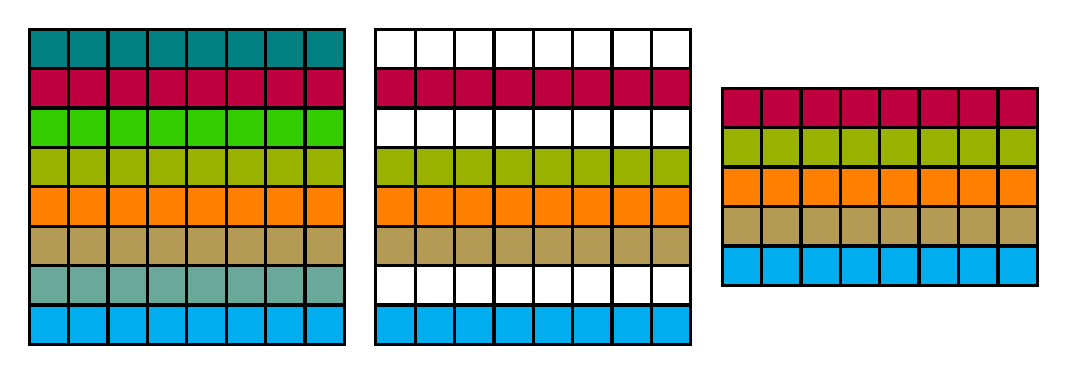
\begin{tikzpicture}
        \filldraw[cyan, draw=black, very thick] (0,0) rectangle (4,0.5);
        \filldraw[cyan!60!orange, draw=black, very thick] (0,0.5) rectangle (4,1);
        \filldraw[cyan!30!orange, draw=black, very thick] (0,1) rectangle (4,1.5);
        \filldraw[orange, draw=black, very thick] (0,1.5) rectangle (4,2);
        \filldraw[orange!60!green, draw=black, very thick] (0,2) rectangle (4,2.5);
        \filldraw[green!80!red, draw=black, very thick] (0,2.5) rectangle (4,3);
        \filldraw[purple, draw=black, very thick] (0,3) rectangle (4,3.5);
        \filldraw[teal, draw=black, very thick] (0,3.5) rectangle (4,4);
        \draw[very thick] (0, 0) -- (0, 4);
        \draw[very thick] (0.5, 0) -- (0.5, 4);
        \draw[very thick] (1, 0) -- (1, 4);
        \draw[very thick] (1.5, 0) -- (1.5, 4);
        \draw[very thick] (2, 0) -- (2, 4);
        \draw[very thick] (2.5, 0) -- (2.5, 4);
        \draw[very thick] (3, 0) -- (3, 4);
        \draw[very thick] (3.5, 0) -- (3.5, 4);
        \filldraw[cyan, draw=black, very thick] (4.4,0) rectangle (8.4,0.5);
        \filldraw[white, draw=black, very thick] (4.4,0.5) rectangle (8.4,1);
        \filldraw[cyan!30!orange, draw=black, very thick] (4.4,1) rectangle (8.4,1.5);
        \filldraw[orange, draw=black, very thick] (4.4,1.5) rectangle (8.4,2);
        \filldraw[orange!60!green, draw=black, very thick] (4.4,2) rectangle (8.4,2.5);
        \filldraw[white, draw=black, very thick] (4.4,2.5) rectangle (8.4,3);
        \filldraw[purple, draw=black, very thick] (4.4,3) rectangle (8.4,3.5);
        \filldraw[white, draw=black, very thick] (4.4,3.5) rectangle (8.4,4);
        \draw[very thick] (4.4, 0) -- (4.4, 4);
        \draw[very thick] (4.9, 0) -- (4.9, 4);
        \draw[very thick] (5.4, 0) -- (5.4, 4);
        \draw[very thick] (5.9, 0) -- (5.9, 4);
        \draw[very thick] (6.4, 0) -- (6.4, 4);
        \draw[very thick] (6.9, 0) -- (6.9, 4);
        \draw[very thick] (7.4, 0) -- (7.4, 4);
        \draw[very thick] (7.9, 0) -- (7.9, 4);
        \filldraw[cyan, draw=black, very thick] (8.8,0.75) rectangle (12.8,1.25);
        \filldraw[cyan!30!orange, draw=black, very thick] (8.8,1.25) rectangle (12.8,1.75);
        \filldraw[orange, draw=black, very thick] (8.8,1.75) rectangle (12.8,2.25);
        \filldraw[orange!60!green, draw=black, very thick] (8.8,2.25) rectangle (12.8,2.75);
        \filldraw[purple, draw=black, very thick] (8.8,2.75) rectangle (12.8,3.25);
        \draw[very thick] (8.8, 0.75) -- (8.8, 3.25);
        \draw[very thick] (9.3, 0.75) -- (9.3, 3.25);
        \draw[very thick] (9.8, 0.75) -- (9.8, 3.25);
        \draw[very thick] (10.3, 0.75) -- (10.3, 3.25);
        \draw[very thick] (10.8, 0.75) -- (10.8, 3.25);
        \draw[very thick] (11.3, 0.75) -- (11.3, 3.25);
        \draw[very thick] (11.8, 0.75) -- (11.8, 3.25);
        \draw[very thick] (12.3, 0.75) -- (12.3, 3.25);
    \end{tikzpicture}
    \caption{Left: $8 \times8$ matrix $U$ . Middle: $8 \times 8$ matrix corresponding to $P_{\Lambda} U$, where
$\Lambda = \{2, 4, 5, 6, 8\}$. Right: $5 \times 8$ matrix corresponding to $P_{\Lambda} U$ (Figure 5.1)} 
    %\label{}
\end{figure}

\begin{figure}
\begin{center}
\begin{tikzpicture}[scale=1.7]

% p = 1
\draw (1.7, 0) -- (4.3, 0);
\draw (3, 1.3) -- (3, -1.3) node[below] {$p = 1$};
\draw[dashed] (2,0) -- (3,1) -- (4,0) -- (3, -1) -- (2,0);
\draw (2, 1.333) -- (4.5,0.5);
\draw (3,1) node {\textbullet};
\draw (3,1) node[above right] {$\hat{x}$};


% p = 2

\draw (5.7, 0) -- (8.3, 0);
\draw (7, 1.3) -- (7, -1.3) node[below] {$p = 2$};
\draw[dashed] (7,0) circle (1);
\draw (6, 1.4) -- (8.5, 0.57);
\draw (7 + 0.32,0.94) node {\textbullet};
\draw (7  + 0.32,0.94) node[above right] {$\hat{x}$};

\end{tikzpicture}
\end{center}
\caption{The $\ell^1$-norm promotes sparsity. (Figure 5.3)}
\end{figure}

\begin{figure}[htbp]
    \centering
    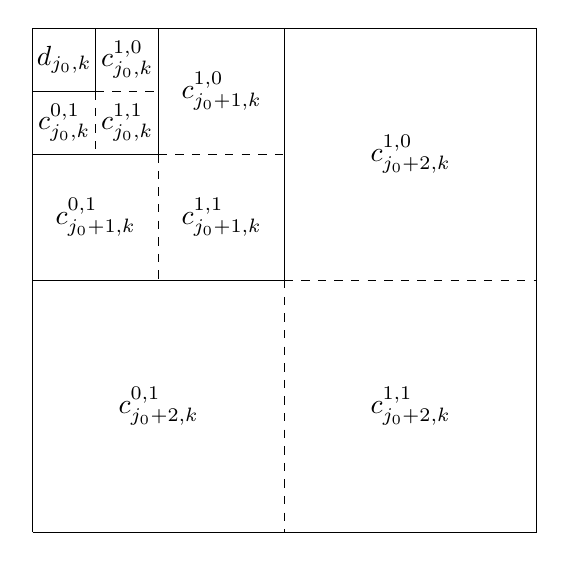
\begin{tikzpicture}[scale=0.8] % Use the scale parameter to adjust size
        \draw (0,0) -- (8,0) -- (8,8) -- (0,8) -- (0,0);
        \draw (0,4) -- (4,4) -- (4,8);
        \draw[dashed] (4,4) -- (8,4);
        \draw[dashed] (4,4) -- (4,0);
        \draw (0,6) -- (2,6) -- (2,8);
        \draw[dashed] (2,6) -- (4,6);
        \draw[dashed] (2,6) -- (2,4);
        \draw (0,7) -- (1,7) -- (1,8);
        \draw[dashed] (1,7) -- (2,7);
        \draw[dashed] (1,7) -- (1,6);
        \node at (2,2) {$c_{j_0+2,k}^{0,1}$};
        \node at (6,2) {$c_{j_0+2,k}^{1,1}$};
        \node at (6,6) {$c_{j_0+2,k}^{1,0}$};
        
        \node at (1,5) {$c_{j_0+1,k}^{0,1}$};
        \node at (3,5) {$c_{j_0+1,k}^{1,1}$};
        \node at (3,7) {$c_{j_0+1,k}^{1,0}$};
        
        \node at (0.5,6.5) {$c_{j_0,k}^{0,1}$};
        \node at (1.5,6.5) {$c_{j_0,k}^{1,1}$};
        \node at (1.5,7.5) {$c_{j_0,k}^{1,0}$};
        \node at (0.5,7.5) {$d_{j_0,k}$};
    \end{tikzpicture}
    \caption{Ordering of wavelet coefficients. (Figure 9.7) }
\end{figure}

\begin{figure}
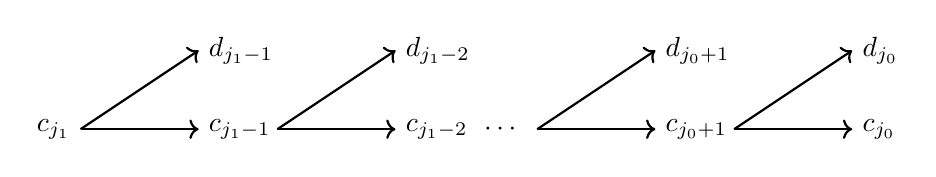
\begin{tikzpicture}[scale=1]
% DWT
\draw[->, thick] (0,0) node[left] {$c_{j_1}$} -- (1.5,0) node[right] {$c_{j_1-1}$};
\draw[->, thick] (0,0)  -- (1.5,1) node[right] {$d_{j_1-1}$};
\draw[->, thick] (2.5,0) -- (4.0,0) node[right] {$c_{j_1-2}$};
\draw[->, thick] (2.5,0) -- (4.0,1) node[right] {$d_{j_1-2}$};
\draw (5.0,0) node[right] {$\cdots$};
\draw[->, thick] (5.8,0) -- (7.3,0) node[right] {$c_{j_0+1}$};
\draw[->, thick] (5.8,0) -- (7.3,1) node[right] {$d_{j_0+1}$};
\draw[->, thick] (8.3,0) -- (9.8,0) node[right] {$c_{j_0}$};
\draw[->, thick] (8.3,0) -- (9.8,1) node[right] {$d_{j_0}$};
\end{tikzpicture}

\vspace{12pt}
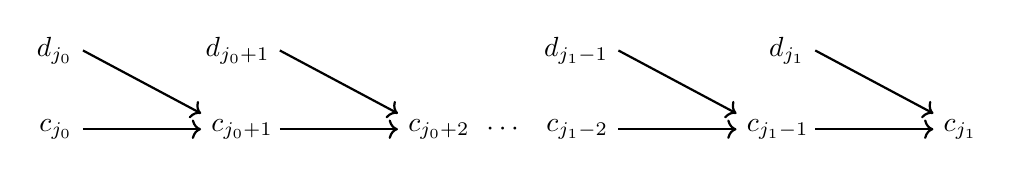
\begin{tikzpicture}[scale=1]
% IDWT
\draw[->, thick] (0,0) node[left] {$c_{j_0}$} -- (1.5,0) node[right] {$c_{j_0+1}$};
\draw[->, thick] (0,1) node[left] {$d_{j_0}$} -- (1.5,0.2) ;
\draw[->, thick] (2.5,0) -- (4.0,0) node[right] {$c_{j_0+2}$};
\draw[->, thick] (2.5,1) node[left] {$d_{j_0+1}$} -- (4.0,0.2) ;
\draw (5.0,0) node[right] {$\cdots$};
\draw[->, thick] (6.8,0) node[left] {$c_{j_{1}-2}$} -- (8.3,0) node[right] {$c_{j_1-1}$};
\draw[->, thick] (6.8,1) node[left] {$d_{j_1-1}$}-- (8.3,0.2) ;
\draw[->, thick] (9.3,0) -- (10.8,0) node[right] {$c_{j_1}$};
\draw[->, thick] (9.3,1) node[left] {$d_{j_1}$}-- (10.8,0.2) ;
\end{tikzpicture}
\caption{Implementation of the DWT (top row) and its inverse (bottom row). (Figure 9.8)}
\label{f:cascade}
\end{figure}

\begin{figure}
 \begin{center}
 \begin{tabular}{@{}cc@{}}    
    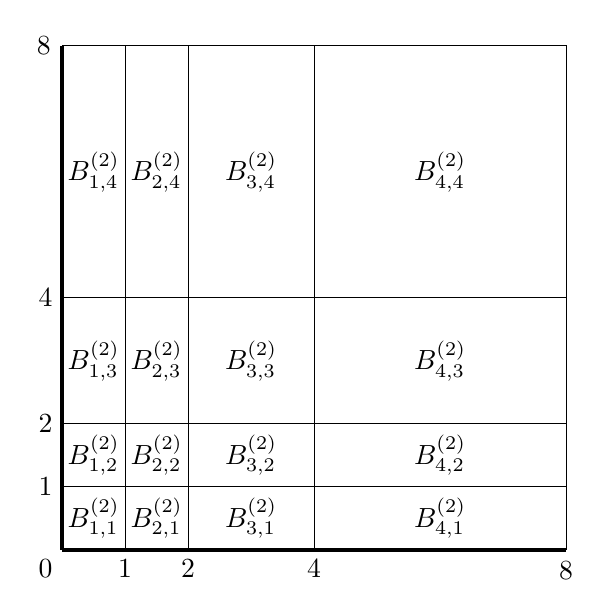
\begin{tikzpicture}[scale=0.8]
    
    	\draw (0,0) node[below left] {0};
	
        \draw[ultra thick] (0,0) -- (8,0)  node[below] {8};
        \draw[ultra thick] (0,0) -- (0,8)  node[left] {8};
        \draw (8,0) -- (8,8) -- (0,8);
        
        \draw (1,0) node[below] {1} -- (1,8);
        \draw (2,0) node[below] {2} -- (2,8);
        \draw (4,0) node[below] {4} -- (4,8);
        
        \draw (0,1) node[left] {1} -- (8,1);
        \draw (0,2) node[left] {2} -- (8,2);
        \draw (0,4) node[left] {4} -- (8,4);
        
        \draw (0.5, 0.5) node {$B_{1,1}^{(2)}$};
        \draw (0.5, 1.5) node {$B_{1,2}^{(2)}$};
        \draw (0.5, 3)   node {$B_{1,3}^{(2)}$};
        \draw (0.5, 6)   node {$B_{1,4}^{(2)}$};
        
        \draw (1.5, 0.5) node {$B_{2,1}^{(2)}$};
        \draw (1.5, 1.5) node {$B_{2,2}^{(2)}$};
        \draw (1.5, 3)   node {$B_{2,3}^{(2)}$};
        \draw (1.5, 6)   node {$B_{2,4}^{(2)}$};

        \draw (3, 0.5) node {$B_{3,1}^{(2)}$};
        \draw (3, 1.5) node {$B_{3,2}^{(2)}$};
        \draw (3, 3)   node {$B_{3,3}^{(2)}$};
        \draw (3, 6)   node {$B_{3,4}^{(2)}$};
        
        \draw (6, 0.5) node {$B_{4,1}^{(2)}$};
        \draw (6, 1.5) node {$B_{4,2}^{(2)}$};
        \draw (6, 3)   node {$B_{4,3}^{(2)}$};
        \draw (6, 6)   node {$B_{4,4}^{(2)}$};
    \end{tikzpicture}
\\
    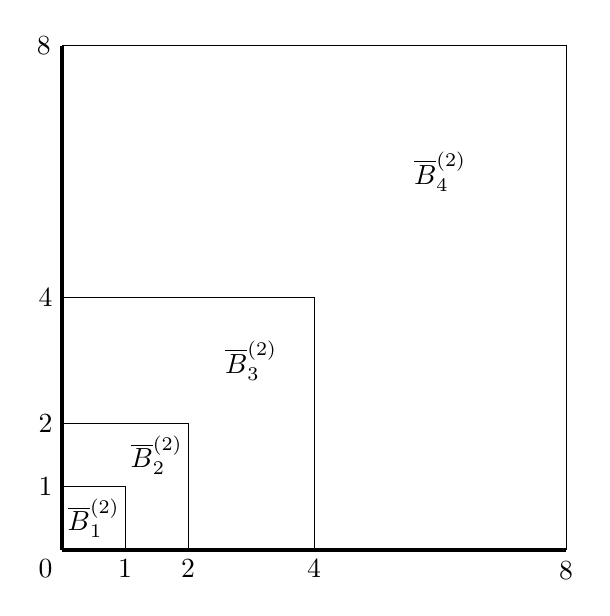
\begin{tikzpicture}[scale=0.8]
    
    	\draw (0,0) node[below left] {0};
    
        \draw[ultra thick] (0,0) -- (8,0)  node[below] {8};
        \draw[ultra thick] (0,0) -- (0,8)  node[left] {8};
        \draw (8,0) -- (8,8) -- (0,8);
        
        \draw (1,0) node[below] {1} -- (1,1) -- (0,1) node[left] {1};
        \draw (2,0) node[below] {2} -- (2,2) -- (0,2) node[left] {2};
        \draw (4,0) node[below] {4} -- (4,4) -- (0,4) node[left] {4};
        
        \draw (0.5, 0.5) node {$\overline{B}_{1}^{(2)}$};
        \draw (1.5, 1.5) node {$\overline{B}_{2}^{(2)}$};
        \draw (3, 3)     node {$\overline{B}_{3}^{(2)}$};
        \draw (6, 6)     node {$\overline{B}_{4}^{(2)}$};
    \end{tikzpicture}

\end{tabular}
\end{center}
\caption{
The sets defining the partitions of $\mathbb{N}^2_0$ with index $j_0 = 0$.  Top: Dyadic anisotropic partition.  Bottom: Dyadic isotropic partition. (Figure 15.1)
}
\end{figure}


\begin{figure}
 \begin{center}
 \begin{tabular}{@{}cc@{}}    

  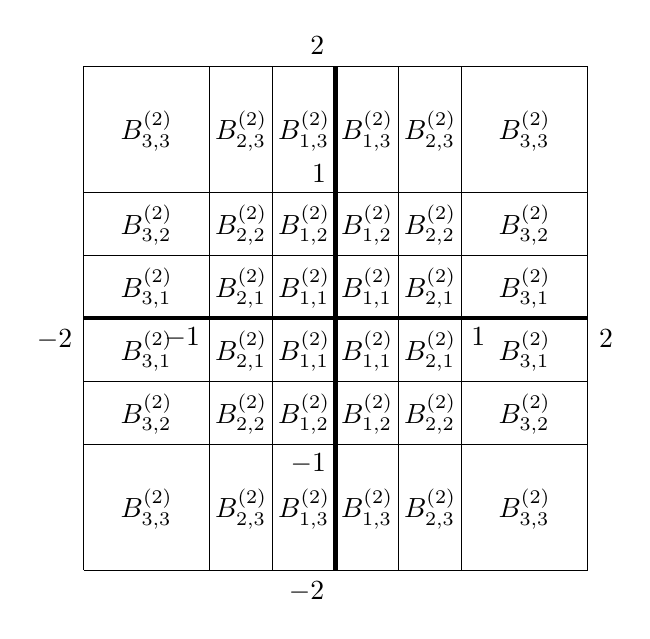
\begin{tikzpicture}[scale=0.8]
        \draw (0,0) -- (8,0) -- (8,8) -- (0,8) -- (0,0);
        
        % Center cross
        \draw[ultra thick] (0,4) node[below left] {$-2$} -- (8,4) node[below right] {$2$};   
        \draw[ultra thick] (4,0) node[below left] {$-2$} -- (4,8) node[above left] {$2$};   
        
        \draw (3,0) -- (3,8);
        \draw (2,0) -- (2,8);
        \draw (5,0) -- (5,8);
        \draw (6,0) -- (6,8);
        
        \draw (0,3) -- (8,3);
        \draw (0,2) -- (8,2);
        \draw (0,5) -- (8,5);
        \draw (0,6) -- (8,6);
        
     %   \draw (4,4) node[below left] {$0$};
        \draw (2,4) node[below left] {$-1$};
        \draw (6,4) node[below right] {$1$};
        \draw (4,6) node[above left] {$1$};
        \draw (4,2) node[below left] {$-1$};
%        \draw (5,4) node[below right] {$\tfrac{1}{2}$};
%        \draw (4,5) node[above left] {$\tfrac{1}{2}$};
        
    
%        \draw[thick, pattern=north east lines, opacity=0.3] (3,3) rectangle (5,5);
        \draw (4.5,4) node[above] {$B_{1,1}^{(2)}$};
        \draw (3.5,4) node[above] {$B_{1,1}^{(2)}$};
        \draw (4.5,3) node[above] {$B_{1,1}^{(2)}$};
        \draw (3.5,3) node[above] {$B_{1,1}^{(2)}$};
        
        \draw (5.5,4) node[above] {$B_{2,1}^{(2)}$};
        \draw (5.5,3) node[above] {$B_{2,1}^{(2)}$};
        \draw (2.5,4) node[above] {$B_{2,1}^{(2)}$};
        \draw (2.5,3) node[above] {$B_{2,1}^{(2)}$};
        
        \draw (3.5,5) node[above] {$B_{1,2}^{(2)}$};
        \draw (4.5,5) node[above] {$B_{1,2}^{(2)}$};
        \draw (3.5,2) node[above] {$B_{1,2}^{(2)}$};
        \draw (4.5,2) node[above] {$B_{1,2}^{(2)}$};
        
        \draw (2.5,5) node[above] {$B_{2,2}^{(2)}$};
        \draw (5.5,5) node[above] {$B_{2,2}^{(2)}$};
        \draw (2.5,2) node[above] {$B_{2,2}^{(2)}$};
        \draw (5.5,2) node[above] {$B_{2,2}^{(2)}$};
        
        \draw (7,6.5) node[above] {$B_{3,3}^{(2)}$};
        \draw (1,6.5) node[above] {$B_{3,3}^{(2)}$};
        \draw (7,0.5) node[above] {$B_{3,3}^{(2)}$};
        \draw (1,0.5) node[above] {$B_{3,3}^{(2)}$};
        
       \draw (7,5.0) node[above] {$B_{3,2}^{(2)}$};
        \draw (1,5.0) node[above] {$B_{3,2}^{(2)}$};
        \draw (7,2.0) node[above] {$B_{3,2}^{(2)}$};
        \draw (1,2.0) node[above] {$B_{3,2}^{(2)}$};
        
        \draw (7,4.0) node[above] {$B_{3,1}^{(2)}$};
        \draw (1,4.0) node[above] {$B_{3,1}^{(2)}$};
        \draw (7,3.0) node[above] {$B_{3,1}^{(2)}$};
        \draw (1,3.0) node[above] {$B_{3,1}^{(2)}$};
        
        \draw (3.5,6.5) node[above] {$B_{1,3}^{(2)}$};
        \draw (4.5,6.5) node[above] {$B_{1,3}^{(2)}$};
        \draw (3.5,0.5) node[above] {$B_{1,3}^{(2)}$};
        \draw (4.5,0.5) node[above] {$B_{1,3}^{(2)}$};
        
        \draw (5.5,6.5) node[above] {$B_{2,3}^{(2)}$};
        \draw (2.5,6.5) node[above] {$B_{2,3}^{(2)}$};
        \draw (5.5,0.5) node[above] {$B_{2,3}^{(2)}$};
        \draw (2.5,0.5) node[above] {$B_{2,3}^{(2)}$};
        
        
    \end{tikzpicture}

\\

 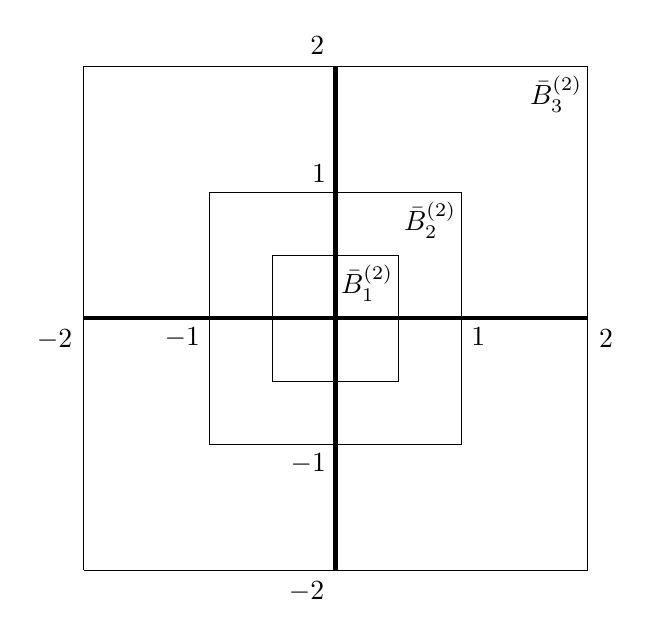
\begin{tikzpicture}[scale=0.8]
        \draw (0,0) -- (8,0) -- (8,8) -- (0,8) -- (0,0);
        
        % Center cross
        \draw[ultra thick] (0,4) node[below left] {$-2$} -- (8,4) node[below right] {$2$};   
        \draw[ultra thick] (4,0) node[below left] {$-2$} -- (4,8) node[above left] {$2$};   
        
        
%        \draw (3,4) node[below left] {$-\tfrac{1}{2}$};
    %    \draw (4,4) node[below left] {$0$};
        \draw (2,4) node[below left] {$-1$};
        \draw (6,4) node[below right] {$1$};
%        \draw (5,4) node[below right] {$\tfrac{1}{2}$};
%        \draw (4,5) node[above left] {$\tfrac{1}{2}$};
        \draw (4,6) node[above left] {$1$};
        \draw (4,2) node[below left] {$-1$};
%        \draw (4,3) node[below left] {$-\tfrac{1}{2}$};
    
        \draw (3,3) rectangle (5,5);
        \draw (2,2) rectangle (6,6);
        
      \draw (4.5,5) node[below] {$\bar{B}_{1}^{(2)}$};
        \draw (5.5,6) node[below] {$\bar{B}_{2}^{(2)}$};
        \draw (7.5,8) node[below] {$\bar{B}_{3}^{(2)}$};
        
    \end{tikzpicture}



\end{tabular}
\end{center}
\caption{
The sets defining the partitions of $\mathbb{Z}^2$ with index $j_0 = 0$.  Top: Dyadic anisotropic partition.  Bottom: Dyadic isotropic partition. (Figure 15.2).
}
\end{figure}


\begin{figure}
    \centering
    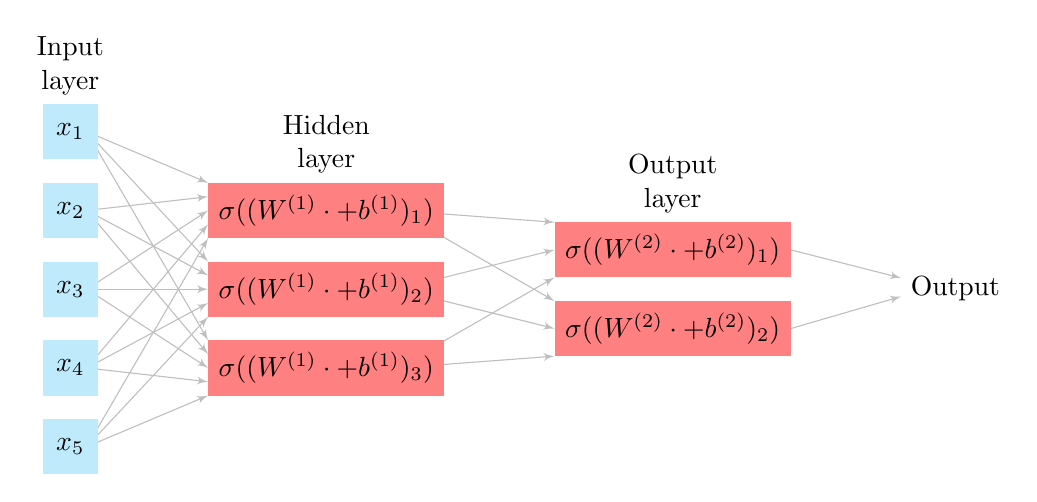
\begin{tikzpicture}[scale=1]
        
        \draw[-latex', black!25] (0.56,4.35) -- (2.1,1.7);
\draw[-latex', black!25] (0.56,4.35) -- (2.1,2.7);
\draw[-latex', black!25] (0.56,4.35) -- (2.1,3.7);
\draw[-latex', black!25] (0.56,3.35) -- (2.1,1.525);
\draw[-latex', black!25] (0.56,3.35) -- (2.1,2.525);
\draw[-latex', black!25] (0.56,3.35) -- (2.1,3.525);
\draw[-latex', black!25] (0.56,2.35) -- (2.1,1.35);
\draw[-latex', black!25] (0.56,2.35) -- (2.1,2.35);
\draw[-latex', black!25] (0.56,2.35) -- (2.1,3.35);
\draw[-latex', black!25] (0.56,1.35) -- (2.1,1.175);
\draw[-latex', black!25] (0.56,1.35) -- (2.1,2.175);
\draw[-latex', black!25] (0.56,1.35) -- (2.1,3.175);
\draw[-latex', black!25] (0.56,0.35) -- (2.1,1);
\draw[-latex', black!25] (0.56,0.35) -- (2.1,2);
\draw[-latex', black!25] (0.56,0.35) -- (2.1,3);
\fill[cyan!25] (0,4) rectangle (0.7,4.7);
\node at (0.35,4.35) {$x_{1}$};
\fill[cyan!25] (0,3) rectangle (0.7,3.7);
\node at (0.35,3.35) {$x_{2}$};
\fill[cyan!25] (0,2) rectangle (0.7,2.7);
\node at (0.35,2.35) {$x_{3}$};
\fill[cyan!25] (0,1) rectangle (0.7,1.7);
\node at (0.35,1.35) {$x_{4}$};
\fill[cyan!25] (0,0) rectangle (0.7,0.7);
\node at (0.35,0.35) {$x_{5}$};
\node[align=center, above] (fds) at (0.35,4.7) {Input\\layer};
\draw[-latex', black!25] (4.5,3.35) -- (6.5,2.2);
\draw[-latex', black!25] (4.5,3.35) -- (6.5,3.2);
\draw[-latex', black!25] (4.5,2.35) -- (6.5,1.85);
\draw[-latex', black!25] (4.5,2.35) -- (6.5,2.85);
\draw[-latex', black!25] (4.5,1.35) -- (6.5,1.5);
\draw[-latex', black!25] (4.5,1.35) -- (6.5,2.5);
\fill[red!50] (2.1,3) rectangle (5.1,3.7);
\node at (3.6,3.35) {$\sigma ( (W^{(1)} \cdot + b^{(1)} )_{1})$};
\fill[red!50] (2.1,2) rectangle (5.1,2.7);
\node at (3.6,2.35) {$\sigma ( (W^{(1)} \cdot + b^{(1)} )_{2})$};
\fill[red!50] (2.1,1) rectangle (5.1,1.7);
\node at (3.6,1.35) {$\sigma ( (W^{(1)} \cdot + b^{(1)} )_{3})$};
\node[align=center, above] (fds) at (3.6,3.7) {Hidden \\layer};
\draw[-latex', black!25] (9.5,2.85) -- (10.9,2.4925);
\fill[red!50] (6.5,2.5) rectangle (9.5,3.2);
\node at (8,2.85) {$\sigma ( (W^{(2)} \cdot + b^{(2)} )_{1})$};
\draw[-latex', black!25] (9.5,1.85) -- (10.9,2.2575);
\fill[red!50] (6.5,1.5) rectangle (9.5,2.2);
\node at (8,1.85) {$\sigma ( (W^{(2)} \cdot + b^{(2)} )_{2})$};
\node[align=center, above] (fds) at (8,3.2) {Output \\layer};
\node[align=center, right] (fds) at (10.9,2.35) {Output};

    \end{tikzpicture}
    \caption{A diagram of a neural network with a single hidden layer and widths
             $n_0 = 5$, $n_1 = 3$ and $n_2 = 2$. (Figure 18.2).} 
\end{figure}

\begin{figure}
    \centering
        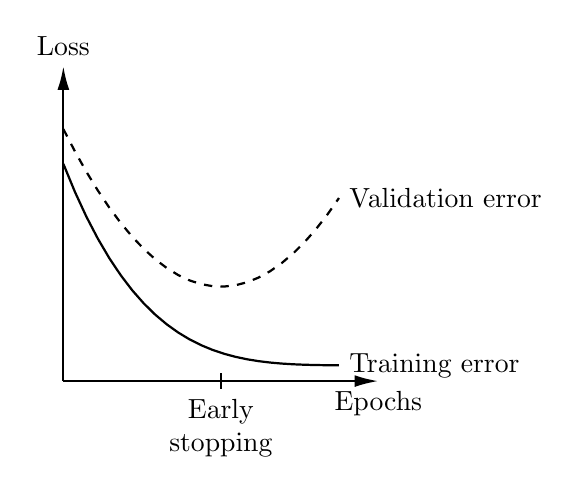
\begin{tikzpicture}
            \draw[thick,-{Latex[length=3mm, width=1.5mm]}] (0,0) -- (4,0) node[below] {Epochs};
            \draw[thick,-{Latex[length=3mm, width=1.5mm]}] (0,0) -- (0,4) node[left, above]  {Loss};

            \draw[thick,domain=0:3.5] plot (\x, {0.01*(\x-4)*(\x-4)*(\x-4)*(\x-4)+0.2}) node[right] {Training error};
            \draw[thick,dashed, domain=0:3.5] plot (\x, {0.5*(\x-2)*(\x-2)+1.2}) node[right] {Validation error};

            \draw[thick,] (2,0.1) -- (2, -0.1) node[below, align=center] {Early \\ stopping}; 
        \end{tikzpicture}
    \caption{Early stopping. (Figure 18.3).} 
\end{figure}

\begin{figure}
    \centering
    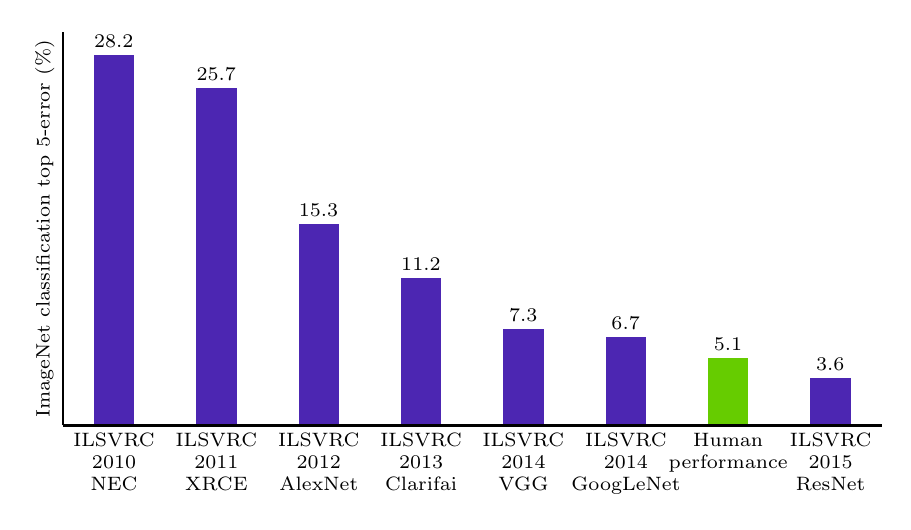
\begin{tikzpicture}[scale=1]
        {\scriptsize
\filldraw[blue!70!orange] (0.4,0) rectangle (0.9,4.7);
\node[above] at (0.6,4.7) {\scriptsize{ 28.2}};
\node[below, align=center] at (0.65,0) { ILSVRC \\ 2010 \\ NEC};
\filldraw[blue!70!orange] (1.7,0) rectangle (2.2,4.28333);
\node[above] at (1.9,4.28333) {\scriptsize{ 25.7}};
\node[below, align=center] at (1.95,0) { ILSVRC \\ 2011 \\ XRCE};
\filldraw[blue!70!orange] (3,0) rectangle (3.5,2.55);
\node[above] at (3.2,2.55) {\scriptsize{ 15.3}};
\node[below, align=center] at (3.25,0) { ILSVRC \\ 2012 \\ AlexNet};
\filldraw[blue!70!orange] (4.3,0) rectangle (4.8,1.86667);
\node[above] at (4.5,1.86667) {\scriptsize{ 11.2}};
\node[below, align=center] at (4.55,0) { ILSVRC \\ 2013 \\ Clarifai};
\filldraw[blue!70!orange] (5.6,0) rectangle (6.1,1.21667);
\node[above] at (5.8,1.21667) {\scriptsize{ 7.3}};
\node[below, align=center] at (5.85,0) { ILSVRC \\ 2014 \\ VGG};
\filldraw[blue!70!orange] (6.9,0) rectangle (7.4,1.11667);
\node[above] at (7.1,1.11667) {\scriptsize{ 6.7}};
\node[below, align=center] at (7.15,0) { ILSVRC \\ 2014 \\ GoogLeNet};
\filldraw[green!60!orange] (8.2,0) rectangle (8.7,0.85);
\node[above] at (8.4,0.85) {\scriptsize{ 5.1}};
\node[below, align=center] at (8.45,0) { Human \\ performance};
\filldraw[blue!70!orange] (9.5,0) rectangle (10,0.6);
\node[above] at (9.7,0.6) {\scriptsize{ 3.6}};
\node[below, align=center] at (9.75,0) { ILSVRC \\ 2015 \\ ResNet};
\draw[thick] (0,0) -- (10.4, 0);
\draw[thick] (0,0) -- (0, 5) node[midway, above, rotate=90] {ImageNet classification top 5-error (\%)};
}

    \end{tikzpicture}
    \caption{Winners of the ImageNet Large Scale Visual Recognition Challenge (ILSVRC). All of the winners since 2012 are based on deep learning.} 
    %\label{}
\end{figure}

\begin{figure}
        \begin{tikzpicture}
            \node at (6,4) {$f(x)< 0$};
            \node at (7.5,2.8) {$f(x)> 0$};
            \draw (0,0) -- (8,4) node[right] {$H$};
            %\draw[->] (4.75,0.5) -- (4,2);

            \draw[-{Latex[length=3mm, width=1.5mm]}] (1,0.5) -- (0.5,1.5) node[above] {$\omega$};

            \draw[-{Latex[length=3mm, width=1.5mm]}] (4.75,0.5) -- (4,2);
            \node at (3.9,2.3) {$x_0+\hat{r}$};
            \node[right, below] at (4.75, 0.5) {$x_0$};
            \fill[black] (4.75,0.5) circle (0.05);
        \end{tikzpicture}
        \caption{Adversarial example for an affine binary classifier. (Figure 18.6).} 
\end{figure}

\begin{figure}
    \centering
    \begin{tikzpicture}[scale=1]
        \draw (7,2) node[below] {$H_1$} -- (4,5);
        \draw (1,1) -- (6,5) node[right] {$H_3$};
        \draw (0,1) -- (7,2.5) node[right] {$H_2$};
        \node at (3.5,2.3) {$P$};
        \fill[black] (5,3) circle (0.05) node[below] {$x_0$};
        \draw[-{Latex[length=3mm, width=1.5mm]}] (5, 3) -- (5.5,3.5) node[right] {$x_0 + \hat{r}$};
    \end{tikzpicture}
\caption{Deep Fool. (Figure (18.7).}
\end{figure}

\begin{figure}
 	\centering
 	    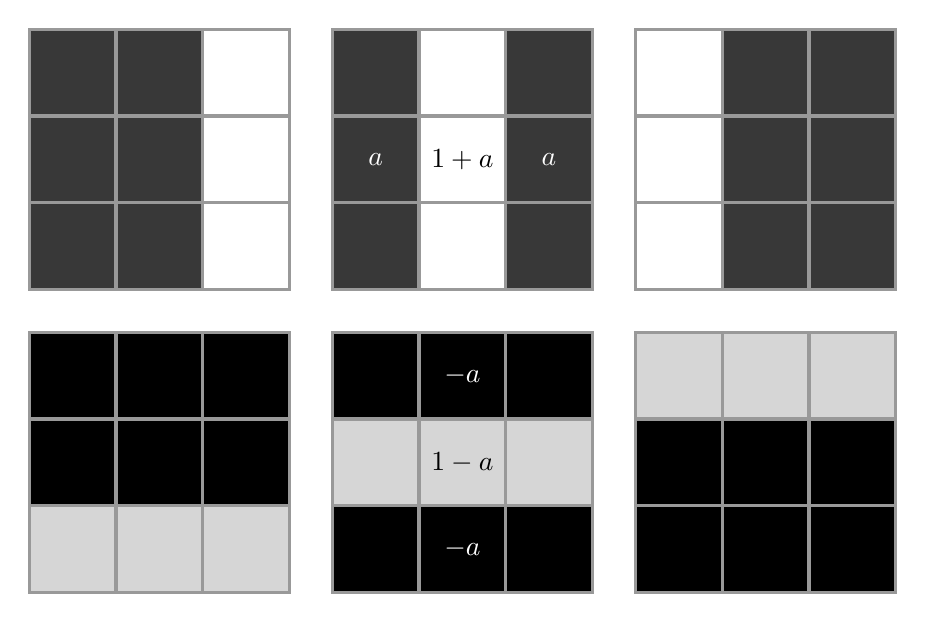
\begin{tikzpicture}[scale=1.1]
       \fill[black!100] (0,1) rectangle (3,3);
 \fill[black!100] (3+0.5,0) rectangle (6+0.5,1);
 \fill[black!100] (3+0.5,2) rectangle (6+0.5,3);
 \fill[black!100] (6+2*0.5,0) rectangle (9+2*0.5,2);
 \fill[black!78] (0,3+0.5) rectangle (2,6+0.5);
 \fill[black!78] (3+0.5,3+0.5) rectangle (4+0.5,6+0.5);
 \fill[black!78] (5+0.5,3+0.5) rectangle (6+0.5,6+0.5);
 \fill[black!78] (7+2*0.5, 3+0.5) rectangle (9+2*0.5,6+0.5);
 \fill[black!16] (0,0) rectangle (3,1);
 \fill[black!16] (3+0.5,1) rectangle (6+0.5,2);
 \fill[black!16] (6+2*0.5,2) rectangle (9+2*0.5,3);
 \draw[very thick, gray!80] (0,0) rectangle (3,3);
 \draw[very thick, gray!80] (3+0.5,0) rectangle (6+0.5,3);
 \draw[very thick, gray!80] (6+1,0) rectangle (9+1,3);
 \draw[very thick, gray!80] (0, 3+0.5) rectangle (3, 6+0.5);
 \draw[very thick, gray!80] (3+0.5, 3+0.5) rectangle (6+0.5, 6+0.5);
 \draw[very thick, gray!80] (6+1, 3+0.5) rectangle (9+1, 6+0.5);
 \draw[very thick, gray!80] (1,0) -- (1,3);
 \draw[very thick, gray!80] (2,0) -- (2,3);
 \draw[very thick, gray!80] (3+0.5+1,0) -- (3+0.5+1,3);
 \draw[very thick, gray!80] (3+0.5+2,0) -- (3+0.5+2,3);
 \draw[very thick, gray!80] (6+2*0.5+1,0) -- (6+2*0.5+1,3);
 \draw[very thick, gray!80] (6+2*0.5+2,0) -- (6+2*0.5+2,3);
 \draw[very thick, gray!80] (1,3+0.5) -- (1,6+0.5);
 \draw[very thick, gray!80] (2,3+0.5) -- (2,6+0.5);
 \draw[very thick, gray!80] (3+0.5+1,3+0.5) -- (3+0.5+1,6+0.5);
 \draw[very thick, gray!80] (3+0.5+2,3+0.5) -- (3+0.5+2,6+0.5);
 \draw[very thick, gray!80] (6+2*0.5+1,3+0.5) -- (6+2*0.5+1,6+0.5);
 \draw[very thick, gray!80] (6+2*0.5+2,3+0.5) -- (6+2*0.5+2,6+0.5);
 \draw[very thick, gray!80] (0, 1) -- (3,1);
 \draw[very thick, gray!80] (0,2) -- (3,2);
 \draw[very thick, gray!80] (0, 3+0.5+1) -- (3, 3+0.5+1);
 \draw[very thick, gray!80] (0, 3+0.5+2) -- (3, 3+0.5+2);
 \draw[very thick, gray!80] (3+0.5, 1) -- (6+0.5,1);
 \draw[very thick, gray!80] (3+0.5,2) -- (6+0.5,2);
 \draw[very thick, gray!80] (3+0.5, 3+0.5+1) -- (6+0.5, 3+0.5+1);
 \draw[very thick, gray!80] (3+0.5, 3+0.5+2) -- (6+0.5, 3+0.5+2);
 \draw[very thick, gray!80] (6+2*0.5, 1) -- (9+2*0.5,1);
 \draw[very thick, gray!80] (6+2*0.5,2) -- (9+2*0.5,2);
 \draw[very thick, gray!80] (6+2*0.5, 3+0.5+1) -- (9+2*0.5, 3+0.5+1);
 \draw[very thick, gray!80] (6+2*0.5, 3+0.5+2) -- (9+2*0.5, 3+0.5+2);
 \draw[white] (4.5+0.5, 0.5)  node {$-a$};
 \draw (4.5+0.5, 1.5)  node {$1-a$};
 \draw[white] (4.5+0.5, 2.5)  node {$-a$};
 \draw[white] (3.5+0.5, 4.5+0.5)  node {$a$};
 \draw[black] (4.5+0.5, 4.5+0.5)  node {$1+a$};
 \draw[white] (5.5+0.5, 4.5+0.5)  node {$a$}; 
     \end{tikzpicture}
\caption{$3 \times 3$ images with either horizontal or vertical stripes. Vertical stripes (top row) are assigned the value $a$ (dark) or $1+a$ (light), and horizontal stripes (bottom row) are assigned the values $-a$ and $1-a$ (bottom row). These images are coloured as follows: $-1/4$ represents black, $1+1/4$ represents white, and numbers in between $-1/4$ and $1+1/4$ represent shades of grey. (Figure 18.9). }
\end{figure}

\begin{figure}[htbp]
    \centering
    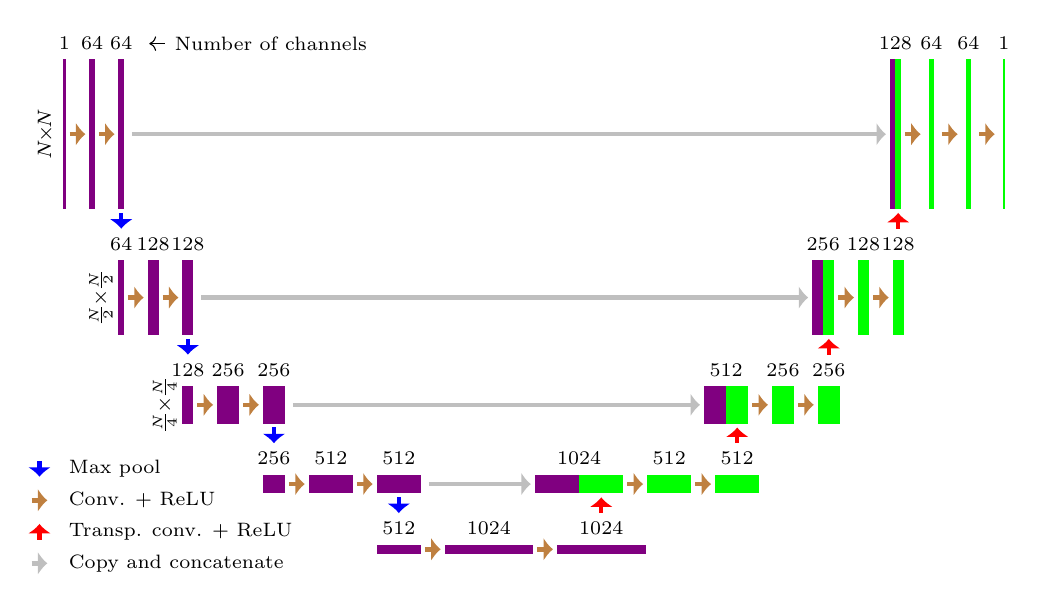
\begin{tikzpicture}[scale=1]
        \fill[violet] (0, 0) rectangle (0.033, -1.9); \node[above]  at (0.0165, 0) {\scriptsize{$1$}};
 \node[rotate=90, above]  at (0, -0.95) {\scriptsize{$N\!\! \times \!\! N$}};
\draw[ultra thick,brown,-{Latex[length=1.2mm,width=3mm]}] (0.083, -0.95) -- (0.283, -0.95);
\fill[violet] (0.333, 0) rectangle (0.4034, -1.9); \node[above]  at (0.3682, 0) {\scriptsize{$64$}};
\draw[ultra thick,brown,-{Latex[length=1.2mm,width=3mm]}] (0.4534, -0.95) -- (0.6534, -0.95);
\fill[violet] (0.7034, 0) rectangle (0.7738, -1.9); \node[above]  at (0.7386, 0) {\scriptsize{$64$}};
\draw[<-] (1.0942,0.2) -- (1.2942,0.2) node[right] {{\scriptsize Number of channels}};
\draw[ultra thick,blue,-{Latex[length=1.2mm,width=3mm]}] (0.7386, -1.95) -- (0.7386, -2.15);
\fill[violet] (0.7034, -2.55) rectangle (0.7738, -3.5); \node[above]  at (0.7386, -2.55) {\scriptsize{$64$}};
 \node[rotate=90, above]  at (0.7534, -3.025) {\scriptsize{$\tfrac{N}{2}\!\! \times \!\!\tfrac{N}{2}$}};
\draw[ultra thick,brown,-{Latex[length=1.2mm,width=3mm]}] (0.8238, -3.025) -- (1.0238, -3.025);
\fill[violet] (1.0738, -2.55) rectangle (1.2146, -3.5); \node[above]  at (1.1442, -2.55) {\scriptsize{$128$}};
\draw[ultra thick,brown,-{Latex[length=1.2mm,width=3mm]}] (1.2646, -3.025) -- (1.4646, -3.025);
\fill[violet] (1.5146, -2.55) rectangle (1.6554, -3.5); \node[above]  at (1.585, -2.55) {\scriptsize{$128$}};
\draw[ultra thick,blue,-{Latex[length=1.2mm,width=3mm]}] (1.585, -3.55) -- (1.585, -3.75);
\fill[violet] (1.5146, -4.15) rectangle (1.6554, -4.625); \node[above]  at (1.585, -4.15) {\scriptsize{$128$}};
 \node[rotate=90, above]  at (1.5646, -4.3875) {\scriptsize{$\tfrac{N}{4}\!\! \times \!\!\tfrac{N}{4}$}};
\draw[ultra thick,brown,-{Latex[length=1.2mm,width=3mm]}] (1.7054, -4.3875) -- (1.9054, -4.3875);
\fill[violet] (1.9554, -4.15) rectangle (2.237, -4.625); \node[above]  at (2.0962, -4.15) {\scriptsize{$256$}};
\draw[ultra thick,brown,-{Latex[length=1.2mm,width=3mm]}] (2.287, -4.3875) -- (2.487, -4.3875);
\fill[violet] (2.537, -4.15) rectangle (2.8186, -4.625); \node[above]  at (2.6778, -4.15) {\scriptsize{$256$}};
\draw[ultra thick,blue,-{Latex[length=1.2mm,width=3mm]}] (2.6778, -4.675) -- (2.6778, -4.875);
\fill[violet] (2.537, -5.275) rectangle (2.8186, -5.5125); \node[above]  at (2.6778, -5.275) {\scriptsize{$256$}};
\draw[ultra thick,brown,-{Latex[length=1.2mm,width=3mm]}] (2.8686, -5.39375) -- (3.0686, -5.39375);
\fill[violet] (3.1186, -5.275) rectangle (3.6818, -5.5125); \node[above]  at (3.4002, -5.275) {\scriptsize{$512$}};
\draw[ultra thick,brown,-{Latex[length=1.2mm,width=3mm]}] (3.7318, -5.39375) -- (3.9318, -5.39375);
\fill[violet] (3.9818, -5.275) rectangle (4.545, -5.5125); \node[above]  at (4.2634, -5.275) {\scriptsize{$512$}};
\draw[ultra thick,blue,-{Latex[length=1.2mm,width=3mm]}] (4.2634, -5.5625) -- (4.2634, -5.7625);
\fill[violet] (3.9818, -6.1625) rectangle (4.545, -6.28125); \node[above]  at (4.2634, -6.1625) {\scriptsize{$512$}};
\draw[ultra thick,brown,-{Latex[length=1.2mm,width=3mm]}] (4.595, -6.22187) -- (4.795, -6.22187);
\fill[violet] (4.845, -6.1625) rectangle (5.9714, -6.28125); \node[above]  at (5.4082, -6.1625) {\scriptsize{$1024$}};
\draw[ultra thick,brown,-{Latex[length=1.2mm,width=3mm]}] (6.0214, -6.22187) -- (6.2214, -6.22187);
\fill[violet] (6.2714, -6.1625) rectangle (7.3978, -6.28125); \node[above]  at (6.8346, -6.1625) {\scriptsize{$1024$}};
\draw[ultra thick,red,-{Latex[length=1.2mm,width=3mm]}] (6.8346, -5.7625) -- (6.8346, -5.5625);
\fill[green] (6.553, -5.275) rectangle (7.1162, -5.5125); \node[above]  at (6.553, -5.275) {\scriptsize{$1024$}};
\fill[violet] (5.9898, -5.275) rectangle (6.553, -5.5125);
\draw[ultra thick,brown,-{Latex[length=1.2mm,width=3mm]}] (7.1662, -5.39375) -- (7.3662, -5.39375);
\fill[green] (7.4162, -5.275) rectangle (7.9794, -5.5125); \node[above]  at (7.6978, -5.275) {\scriptsize{$512$}};
\draw[ultra thick,brown,-{Latex[length=1.2mm,width=3mm]}] (8.0294, -5.39375) -- (8.2294, -5.39375);
\fill[green] (8.2794, -5.275) rectangle (8.8426, -5.5125); \node[above]  at (8.561, -5.275) {\scriptsize{$512$}};
\draw[ultra thick,red,-{Latex[length=1.2mm,width=3mm]}] (8.561, -4.875) -- (8.561, -4.675);
\fill[green] (8.4202, -4.15) rectangle (8.7018, -4.625); \node[above]  at (8.4202, -4.15) {\scriptsize{$512$}};
\fill[violet] (8.1386, -4.15) rectangle (8.4202, -4.625);
\draw[ultra thick,brown,-{Latex[length=1.2mm,width=3mm]}] (8.7518, -4.3875) -- (8.9518, -4.3875);
\fill[green] (9.0018, -4.15) rectangle (9.2834, -4.625); \node[above]  at (9.1426, -4.15) {\scriptsize{$256$}};
\draw[ultra thick,brown,-{Latex[length=1.2mm,width=3mm]}] (9.3334, -4.3875) -- (9.5334, -4.3875);
\fill[green] (9.5834, -4.15) rectangle (9.865, -4.625); \node[above]  at (9.7242, -4.15) {\scriptsize{$256$}};
\draw[ultra thick,red,-{Latex[length=1.2mm,width=3mm]}] (9.7242, -3.75) -- (9.7242, -3.55);
\fill[green] (9.6538, -2.55) rectangle (9.7946, -3.5); \node[above]  at (9.6538, -2.55) {\scriptsize{$256$}};
\fill[violet] (9.513, -2.55) rectangle (9.6538, -3.5);
\draw[ultra thick,brown,-{Latex[length=1.2mm,width=3mm]}] (9.8446, -3.025) -- (10.0446, -3.025);
\fill[green] (10.0946, -2.55) rectangle (10.2354, -3.5); \node[above]  at (10.165, -2.55) {\scriptsize{$128$}};
\draw[ultra thick,brown,-{Latex[length=1.2mm,width=3mm]}] (10.2854, -3.025) -- (10.4854, -3.025);
\fill[green] (10.5354, -2.55) rectangle (10.6762, -3.5); \node[above]  at (10.6058, -2.55) {\scriptsize{$128$}};
\draw[ultra thick,red,-{Latex[length=1.2mm,width=3mm]}] (10.6058, -2.15) -- (10.6058, -1.95);
\fill[green] (10.5706, 0) rectangle (10.641, -1.9); \node[above]  at (10.5706, 0) {\scriptsize{$128$}};
\fill[violet] (10.5002, 0) rectangle (10.5706, -1.9);
\draw[ultra thick,brown,-{Latex[length=1.2mm,width=3mm]}] (10.691, -0.95) -- (10.891, -0.95);
\fill[green] (10.991, 0) rectangle (11.0614, -1.9); \node[above]  at (11.0262, 0) {\scriptsize{$64$}};
\draw[ultra thick,brown,-{Latex[length=1.2mm,width=3mm]}] (11.1614, -0.95) -- (11.3614, -0.95);
\fill[green] (11.4614, 0) rectangle (11.5318, -1.9); \node[above]  at (11.4966, 0) {\scriptsize{$64$}};
\draw[ultra thick,brown,-{Latex[length=1.2mm,width=3mm]}] (11.6318, -0.95) -- (11.8318, -0.95);
\fill[green] (11.9318, 0) rectangle (11.9648, -1.9); \node[above]  at (11.9483, 0) {\scriptsize{$1$}};
\draw[ultra thick,lightgray,-{Latex[length=1.2mm,width=3mm]}] (0.8738, -0.95) -- (10.4502, -0.95);
\draw[ultra thick,lightgray,-{Latex[length=1.2mm,width=3mm]}] (1.7554, -3.025) -- (9.463, -3.025);
\draw[ultra thick,lightgray,-{Latex[length=1.2mm,width=3mm]}] (2.9186, -4.3875) -- (8.0886, -4.3875);
\draw[ultra thick,lightgray,-{Latex[length=1.2mm,width=3mm]}] (4.645, -5.39375) -- (5.9398, -5.39375);
\draw[ultra thick,blue,-{Latex[length=1.2mm,width=3mm]}] (-0.3, -5.1) -- (-0.3, -5.3);
\node[right] at (-0.05,-5.2) {\scriptsize{Max pool}};
\draw[ultra thick,brown,-{Latex[length=1.2mm,width=3mm]}] (-0.4, -5.6) -- (-0.2, -5.6);
\node[right] at (-0.05,-5.6) {\scriptsize{Conv. + ReLU}};
\draw[ultra thick,red,-{Latex[length=1.2mm,width=3mm]}] (-0.3, -6.1) -- (-0.3, -5.9);
\node[right] at (-0.05,-6) {\scriptsize{Transp. conv. + ReLU}};
\draw[ultra thick,lightgray,-{Latex[length=1.2mm,width=3mm]}] (-0.4, -6.4) -- (-0.2, -6.4);
\node[right] at (-0.05,-6.4) {\scriptsize{Copy and concatenate}};

    \end{tikzpicture}
    \caption{U-Net. (Figure 19.4).} 
    %\label{}
\end{figure}

\begin{figure}
    \centering
    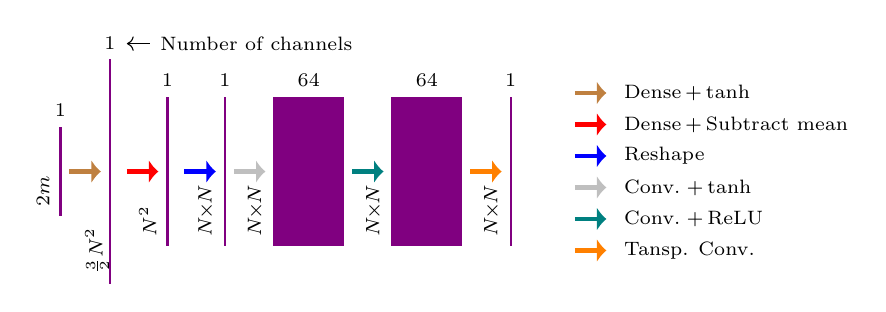
\begin{tikzpicture}[scale=1]
        \fill[violet] (0, 0.57) rectangle (0.03, -0.57); \node[above]  at (0.015, 0.57) {\scriptsize{$1$}};
 \node[rotate=90, above right]  at (0, -0.57) {\scriptsize{$2m$}};
\draw[ultra thick,brown,-{Latex[length=1.2mm,width=3mm]}] (0.13, 0) -- (0.53, 0);
\fill[violet] (0.63, 1.425) rectangle (0.66, -1.425); \node[above]  at (0.645, 1.425) {\scriptsize{$1$}};
 \node[rotate=90, above right]  at (0.76, -1.425) {\scriptsize{$\tfrac{3}{2}N^2$}};
\draw[<-] (0.86,1.6245) -- (1.16,1.6245) node[right] {{\scriptsize Number of channels}};
\draw[ultra thick,red,-{Latex[length=1.2mm,width=3mm]}] (0.86, 0) -- (1.26, 0);
\fill[violet] (1.36, 0.95) rectangle (1.39, -0.95); \node[above]  at (1.375, 0.95) {\scriptsize{$1$}};
 \node[rotate=90, above right]  at (1.36, -0.95) {\scriptsize{$N^2$}};
\draw[ultra thick,blue,-{Latex[length=1.2mm,width=3mm]}] (1.59, 0) -- (1.99, 0);
\fill[violet] (2.09, 0.95) rectangle (2.12, -0.95); \node[above]  at (2.105, 0.95) {\scriptsize{$1$}};
 \node[rotate=90, above right]  at (2.09, -0.95) {\scriptsize{$N\!\!\times \!\! N$}};
\draw[ultra thick,lightgray,-{Latex[length=1.2mm,width=3mm]}] (2.22, 0) -- (2.62, 0);
\fill[violet] (2.72, 0.95) rectangle (3.62, -0.95); \node[above]  at (3.17, 0.95) {\scriptsize{$64$}};
 \node[rotate=90, above right]  at (2.72, -0.95) {\scriptsize{$N\!\!\times \!\! N$}};
\draw[ultra thick,teal,-{Latex[length=1.2mm,width=3mm]}] (3.72, 0) -- (4.12, 0);
\fill[violet] (4.22, 0.95) rectangle (5.12, -0.95); \node[above]  at (4.67, 0.95) {\scriptsize{$64$}};
 \node[rotate=90, above right]  at (4.22, -0.95) {\scriptsize{$N\!\!\times \!\! N$}};
\draw[ultra thick,orange,-{Latex[length=1.2mm,width=3mm]}] (5.22, 0) -- (5.62, 0);
\fill[violet] (5.72, 0.95) rectangle (5.75, -0.95); \node[above]  at (5.735, 0.95) {\scriptsize{$1$}};
 \node[rotate=90, above right]  at (5.72, -0.95) {\scriptsize{$N\!\!\times \!\! N$}};
\draw[ultra thick,brown,-{Latex[length=1.2mm,width=3mm]}] (6.55, 0.9975) -- (6.95, 0.9975);
\node[right] at (7.05,0.9975) {\scriptsize{Dense \!+\! $\tanh$}};
\draw[ultra thick,red,-{Latex[length=1.2mm,width=3mm]}] (6.55, 0.5975) -- (6.95, 0.5975);
\node[right] at (7.05,0.5975) {\scriptsize{Dense \!+\! Subtract mean}};
\draw[ultra thick,blue,-{Latex[length=1.2mm,width=3mm]}] (6.55, 0.1975) -- (6.95, 0.1975);
\node[right] at (7.05,0.1975) {\scriptsize{Reshape}};
\draw[ultra thick,lightgray,-{Latex[length=1.2mm,width=3mm]}] (6.55, -0.2025) -- (6.95, -0.2025);
\node[right] at (7.05,-0.2025) {\scriptsize{Conv. \!+\! $\tanh$}};
\draw[ultra thick,teal,-{Latex[length=1.2mm,width=3mm]}] (6.55, -0.6025) -- (6.95, -0.6025);
\node[right] at (7.05,-0.6025) {\scriptsize{Conv. \!+\! ReLU}};
\draw[ultra thick,orange,-{Latex[length=1.2mm,width=3mm]}] (6.55, -1.0025) -- (6.95, -1.0025);
\node[right] at (7.05,-1.0025) {\scriptsize{Tansp. Conv. }};

    \end{tikzpicture}
    \caption{Automap. (Figure 19.5).} 
    %\label{}
\end{figure}



\begin{figure}[htbp]
\begin{center}
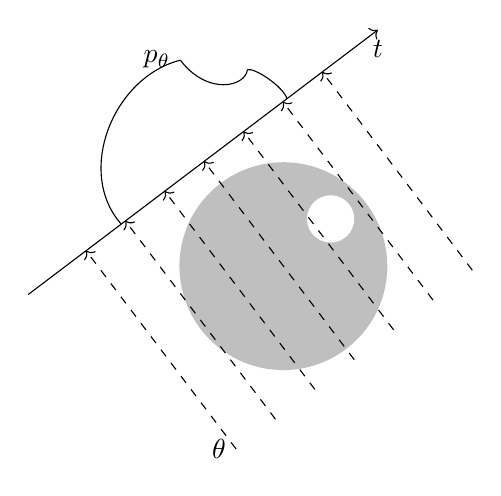
\begin{tikzpicture}[scale=1.2]
    \fill[lightgray] (5,5) circle (1.1);
    \fill[white] (5.5,5.5) circle (0.25);
    \draw[->] (2.3,4.7)  -- (6,7.5) node[below=0.15] {$t$}; 
    %\draw (4, 2.68) -- (7, 4.95);
    \draw (3.28, 5.45) .. controls (2.8,6) and  (3.2, 7) .. (3.91, 7.18) node[above=0.2, left=0.2] {$p_{\theta}$};
    \draw (3.91, 7.18) .. controls (4.2,6.8) and (4.6,6.9) .. (4.62, 7.08);    
    \draw (4.62, 7.08) .. controls (4.7, 7.1) and (5., 6.9) .. (5.04, 6.77);

    \draw[dashed, ->] (4.5, 3.06486) node[left=0.2] {$\theta$} -- (2.91208, 5.16319);
    \draw[dashed, ->] (4.91667, 3.38018) -- (3.32874, 5.47851);
    \draw[dashed, ->] (5.33333, 3.6955) -- (3.74541, 5.79382);
    \draw[dashed, ->] (5.75, 4.01081) -- (4.16208, 6.10914);
    \draw[dashed, ->] (6.16667, 4.32613) -- (4.57874, 6.42445);
    \draw[dashed, ->] (6.58333, 4.64144) -- (4.99541, 6.73977);
    \draw[dashed, ->] (7, 4.95676) -- (5.41208, 7.05508);
\end{tikzpicture}
\end{center}
\caption{(\textbf{Not used in the book}). Radon transform (the graph of $p_{\theta}$ is not mathematically accurate).}
\end{figure}


\begin{figure}[htbp]
    \centering
    \begin{tikzpicture}[scale=1.5]
        \draw (-1.2, 0) -- (1.2, 0);
\draw (0, -1.2) -- (0, 1.2);
\draw[dashed] (0, -0.769231) -- (-0.769231,0) -- (0, 0.769231) -- (0.769231, 0) -- (0,-0.769231);
\draw (-0.3, 1) -- (1.26, -0.2);
\draw[-{Latex[length=2mm, width=1mm]}] (0.63, 0.284615)  -- (1.13, 0.934615) node[midway, right] {$A = [1,~~1+\epsilon]$};
\draw (2.1, 0) -- (4.5, 0);
\draw (3.3, -1.2) -- (3.3, 1.2);
\draw[dashed] (3.3, -1) -- (2.3,0) -- (3.3, 1) -- (4.3, 0) -- (3.3,-1);
\draw (3.6, 1) -- (4.44, -0.2);
\draw[-{Latex[length=2mm, width=1mm]}] (3.72857, 0.816327)  -- (4.22857, 1.16633) node[above, right] {$A = [1,~~1-\epsilon]$};

    \end{tikzpicture}
    \caption{(\textbf{Not used in the book}). Instability $\ell^1$-minimisation.} 
    %\label{}
\end{figure}

\begin{figure}
\centering
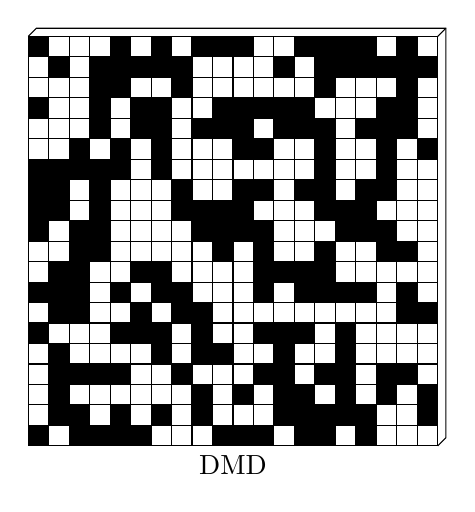
\begin{tikzpicture}[scale=0.65]
    \draw (0,0) rectangle (8,8);
\draw (0.4,0) -- (0.4, 8);
\draw (0,0.4) -- (8, 0.4);
\draw (0.8,0) -- (0.8, 8);
\draw (0,0.8) -- (8, 0.8);
\draw (1.2,0) -- (1.2, 8);
\draw (0,1.2) -- (8, 1.2);
\draw (1.6,0) -- (1.6, 8);
\draw (0,1.6) -- (8, 1.6);
\draw (2,0) -- (2, 8);
\draw (0,2) -- (8, 2);
\draw (2.4,0) -- (2.4, 8);
\draw (0,2.4) -- (8, 2.4);
\draw (2.8,0) -- (2.8, 8);
\draw (0,2.8) -- (8, 2.8);
\draw (3.2,0) -- (3.2, 8);
\draw (0,3.2) -- (8, 3.2);
\draw (3.6,0) -- (3.6, 8);
\draw (0,3.6) -- (8, 3.6);
\draw (4,0) -- (4, 8);
\draw (0,4) -- (8, 4);
\draw (4.4,0) -- (4.4, 8);
\draw (0,4.4) -- (8, 4.4);
\draw (4.8,0) -- (4.8, 8);
\draw (0,4.8) -- (8, 4.8);
\draw (5.2,0) -- (5.2, 8);
\draw (0,5.2) -- (8, 5.2);
\draw (5.6,0) -- (5.6, 8);
\draw (0,5.6) -- (8, 5.6);
\draw (6,0) -- (6, 8);
\draw (0,6) -- (8, 6);
\draw (6.4,0) -- (6.4, 8);
\draw (0,6.4) -- (8, 6.4);
\draw (6.8,0) -- (6.8, 8);
\draw (0,6.8) -- (8, 6.8);
\draw (7.2,0) -- (7.2, 8);
\draw (0,7.2) -- (8, 7.2);
\draw (7.6,0) -- (7.6, 8);
\draw (0,7.6) -- (8, 7.6);
\filldraw[black] (0, 0) rectangle (0.4, 0.4);
\filldraw[black] (0, 2) rectangle (0.4, 2.4);
\filldraw[black] (0, 2.8) rectangle (0.4, 3.2);
\filldraw[black] (0, 4) rectangle (0.4, 4.4);
\filldraw[black] (0, 4.4) rectangle (0.4, 4.8);
\filldraw[black] (0, 4.8) rectangle (0.4, 5.2);
\filldraw[black] (0, 5.2) rectangle (0.4, 5.6);
\filldraw[black] (0, 6.4) rectangle (0.4, 6.8);
\filldraw[black] (0, 7.6) rectangle (0.4, 8);
\filldraw[black] (0.4, 0.4) rectangle (0.8, 0.8);
\filldraw[black] (0.4, 0.8) rectangle (0.8, 1.2);
\filldraw[black] (0.4, 1.2) rectangle (0.8, 1.6);
\filldraw[black] (0.4, 1.6) rectangle (0.8, 2);
\filldraw[black] (0.4, 2.4) rectangle (0.8, 2.8);
\filldraw[black] (0.4, 2.8) rectangle (0.8, 3.2);
\filldraw[black] (0.4, 3.2) rectangle (0.8, 3.6);
\filldraw[black] (0.4, 4.4) rectangle (0.8, 4.8);
\filldraw[black] (0.4, 4.8) rectangle (0.8, 5.2);
\filldraw[black] (0.4, 5.2) rectangle (0.8, 5.6);
\filldraw[black] (0.4, 7.2) rectangle (0.8, 7.6);
\filldraw[black] (0.8, 0) rectangle (1.2, 0.4);
\filldraw[black] (0.8, 0.4) rectangle (1.2, 0.8);
\filldraw[black] (0.8, 1.2) rectangle (1.2, 1.6);
\filldraw[black] (0.8, 2.4) rectangle (1.2, 2.8);
\filldraw[black] (0.8, 2.8) rectangle (1.2, 3.2);
\filldraw[black] (0.8, 3.2) rectangle (1.2, 3.6);
\filldraw[black] (0.8, 3.6) rectangle (1.2, 4);
\filldraw[black] (0.8, 4) rectangle (1.2, 4.4);
\filldraw[black] (0.8, 5.2) rectangle (1.2, 5.6);
\filldraw[black] (0.8, 5.6) rectangle (1.2, 6);
\filldraw[black] (1.2, 0) rectangle (1.6, 0.4);
\filldraw[black] (1.2, 1.2) rectangle (1.6, 1.6);
\filldraw[black] (1.2, 3.6) rectangle (1.6, 4);
\filldraw[black] (1.2, 4) rectangle (1.6, 4.4);
\filldraw[black] (1.2, 4.4) rectangle (1.6, 4.8);
\filldraw[black] (1.2, 4.8) rectangle (1.6, 5.2);
\filldraw[black] (1.2, 5.2) rectangle (1.6, 5.6);
\filldraw[black] (1.2, 6) rectangle (1.6, 6.4);
\filldraw[black] (1.2, 6.4) rectangle (1.6, 6.8);
\filldraw[black] (1.2, 6.8) rectangle (1.6, 7.2);
\filldraw[black] (1.2, 7.2) rectangle (1.6, 7.6);
\filldraw[black] (1.6, 0) rectangle (2, 0.4);
\filldraw[black] (1.6, 0.4) rectangle (2, 0.8);
\filldraw[black] (1.6, 1.2) rectangle (2, 1.6);
\filldraw[black] (1.6, 2) rectangle (2, 2.4);
\filldraw[black] (1.6, 2.8) rectangle (2, 3.2);
\filldraw[black] (1.6, 5.2) rectangle (2, 5.6);
\filldraw[black] (1.6, 5.6) rectangle (2, 6);
\filldraw[black] (1.6, 6.8) rectangle (2, 7.2);
\filldraw[black] (1.6, 7.2) rectangle (2, 7.6);
\filldraw[black] (1.6, 7.6) rectangle (2, 8);
\filldraw[black] (2, 0) rectangle (2.4, 0.4);
\filldraw[black] (2, 2) rectangle (2.4, 2.4);
\filldraw[black] (2, 2.4) rectangle (2.4, 2.8);
\filldraw[black] (2, 3.2) rectangle (2.4, 3.6);
\filldraw[black] (2, 6) rectangle (2.4, 6.4);
\filldraw[black] (2, 6.4) rectangle (2.4, 6.8);
\filldraw[black] (2, 7.2) rectangle (2.4, 7.6);
\filldraw[black] (2.4, 0.4) rectangle (2.8, 0.8);
\filldraw[black] (2.4, 1.6) rectangle (2.8, 2);
\filldraw[black] (2.4, 2) rectangle (2.8, 2.4);
\filldraw[black] (2.4, 2.8) rectangle (2.8, 3.2);
\filldraw[black] (2.4, 3.2) rectangle (2.8, 3.6);
\filldraw[black] (2.4, 5.2) rectangle (2.8, 5.6);
\filldraw[black] (2.4, 5.6) rectangle (2.8, 6);
\filldraw[black] (2.4, 6) rectangle (2.8, 6.4);
\filldraw[black] (2.4, 6.4) rectangle (2.8, 6.8);
\filldraw[black] (2.4, 7.2) rectangle (2.8, 7.6);
\filldraw[black] (2.4, 7.6) rectangle (2.8, 8);
\filldraw[black] (2.8, 1.2) rectangle (3.2, 1.6);
\filldraw[black] (2.8, 2.4) rectangle (3.2, 2.8);
\filldraw[black] (2.8, 2.8) rectangle (3.2, 3.2);
\filldraw[black] (2.8, 4.4) rectangle (3.2, 4.8);
\filldraw[black] (2.8, 4.8) rectangle (3.2, 5.2);
\filldraw[black] (2.8, 6.8) rectangle (3.2, 7.2);
\filldraw[black] (2.8, 7.2) rectangle (3.2, 7.6);
\filldraw[black] (3.2, 0.4) rectangle (3.6, 0.8);
\filldraw[black] (3.2, 0.8) rectangle (3.6, 1.2);
\filldraw[black] (3.2, 1.6) rectangle (3.6, 2);
\filldraw[black] (3.2, 2) rectangle (3.6, 2.4);
\filldraw[black] (3.2, 2.4) rectangle (3.6, 2.8);
\filldraw[black] (3.2, 4) rectangle (3.6, 4.4);
\filldraw[black] (3.2, 4.4) rectangle (3.6, 4.8);
\filldraw[black] (3.2, 6) rectangle (3.6, 6.4);
\filldraw[black] (3.2, 7.6) rectangle (3.6, 8);
\filldraw[black] (3.6, 0) rectangle (4, 0.4);
\filldraw[black] (3.6, 1.6) rectangle (4, 2);
\filldraw[black] (3.6, 3.6) rectangle (4, 4);
\filldraw[black] (3.6, 4) rectangle (4, 4.4);
\filldraw[black] (3.6, 4.4) rectangle (4, 4.8);
\filldraw[black] (3.6, 6) rectangle (4, 6.4);
\filldraw[black] (3.6, 6.4) rectangle (4, 6.8);
\filldraw[black] (3.6, 7.6) rectangle (4, 8);
\filldraw[black] (4, 0) rectangle (4.4, 0.4);
\filldraw[black] (4, 0.8) rectangle (4.4, 1.2);
\filldraw[black] (4, 4) rectangle (4.4, 4.4);
\filldraw[black] (4, 4.4) rectangle (4.4, 4.8);
\filldraw[black] (4, 4.8) rectangle (4.4, 5.2);
\filldraw[black] (4, 5.6) rectangle (4.4, 6);
\filldraw[black] (4, 6) rectangle (4.4, 6.4);
\filldraw[black] (4, 6.4) rectangle (4.4, 6.8);
\filldraw[black] (4, 7.6) rectangle (4.4, 8);
\filldraw[black] (4.4, 0) rectangle (4.8, 0.4);
\filldraw[black] (4.4, 1.2) rectangle (4.8, 1.6);
\filldraw[black] (4.4, 2) rectangle (4.8, 2.4);
\filldraw[black] (4.4, 2.8) rectangle (4.8, 3.2);
\filldraw[black] (4.4, 3.2) rectangle (4.8, 3.6);
\filldraw[black] (4.4, 3.6) rectangle (4.8, 4);
\filldraw[black] (4.4, 4) rectangle (4.8, 4.4);
\filldraw[black] (4.4, 4.8) rectangle (4.8, 5.2);
\filldraw[black] (4.4, 5.6) rectangle (4.8, 6);
\filldraw[black] (4.4, 6.4) rectangle (4.8, 6.8);
\filldraw[black] (4.8, 0.4) rectangle (5.2, 0.8);
\filldraw[black] (4.8, 0.8) rectangle (5.2, 1.2);
\filldraw[black] (4.8, 1.2) rectangle (5.2, 1.6);
\filldraw[black] (4.8, 1.6) rectangle (5.2, 2);
\filldraw[black] (4.8, 2) rectangle (5.2, 2.4);
\filldraw[black] (4.8, 3.2) rectangle (5.2, 3.6);
\filldraw[black] (4.8, 6) rectangle (5.2, 6.4);
\filldraw[black] (4.8, 6.4) rectangle (5.2, 6.8);
\filldraw[black] (4.8, 7.2) rectangle (5.2, 7.6);
\filldraw[black] (5.2, 0) rectangle (5.6, 0.4);
\filldraw[black] (5.2, 0.4) rectangle (5.6, 0.8);
\filldraw[black] (5.2, 0.8) rectangle (5.6, 1.2);
\filldraw[black] (5.2, 2) rectangle (5.6, 2.4);
\filldraw[black] (5.2, 2.8) rectangle (5.6, 3.2);
\filldraw[black] (5.2, 3.2) rectangle (5.6, 3.6);
\filldraw[black] (5.2, 4.8) rectangle (5.6, 5.2);
\filldraw[black] (5.2, 6) rectangle (5.6, 6.4);
\filldraw[black] (5.2, 6.4) rectangle (5.6, 6.8);
\filldraw[black] (5.2, 7.6) rectangle (5.6, 8);
\filldraw[black] (5.6, 0) rectangle (6, 0.4);
\filldraw[black] (5.6, 0.4) rectangle (6, 0.8);
\filldraw[black] (5.6, 1.2) rectangle (6, 1.6);
\filldraw[black] (5.6, 2.8) rectangle (6, 3.2);
\filldraw[black] (5.6, 3.2) rectangle (6, 3.6);
\filldraw[black] (5.6, 3.6) rectangle (6, 4);
\filldraw[black] (5.6, 4.4) rectangle (6, 4.8);
\filldraw[black] (5.6, 4.8) rectangle (6, 5.2);
\filldraw[black] (5.6, 5.2) rectangle (6, 5.6);
\filldraw[black] (5.6, 5.6) rectangle (6, 6);
\filldraw[black] (5.6, 6) rectangle (6, 6.4);
\filldraw[black] (5.6, 6.8) rectangle (6, 7.2);
\filldraw[black] (5.6, 7.2) rectangle (6, 7.6);
\filldraw[black] (5.6, 7.6) rectangle (6, 8);
\filldraw[black] (6, 0.4) rectangle (6.4, 0.8);
\filldraw[black] (6, 0.8) rectangle (6.4, 1.2);
\filldraw[black] (6, 1.2) rectangle (6.4, 1.6);
\filldraw[black] (6, 1.6) rectangle (6.4, 2);
\filldraw[black] (6, 2) rectangle (6.4, 2.4);
\filldraw[black] (6, 2.8) rectangle (6.4, 3.2);
\filldraw[black] (6, 4) rectangle (6.4, 4.4);
\filldraw[black] (6, 4.4) rectangle (6.4, 4.8);
\filldraw[black] (6, 7.2) rectangle (6.4, 7.6);
\filldraw[black] (6, 7.6) rectangle (6.4, 8);
\filldraw[black] (6.4, 0) rectangle (6.8, 0.4);
\filldraw[black] (6.4, 0.4) rectangle (6.8, 0.8);
\filldraw[black] (6.4, 2.8) rectangle (6.8, 3.2);
\filldraw[black] (6.4, 4) rectangle (6.8, 4.4);
\filldraw[black] (6.4, 4.4) rectangle (6.8, 4.8);
\filldraw[black] (6.4, 4.8) rectangle (6.8, 5.2);
\filldraw[black] (6.4, 6) rectangle (6.8, 6.4);
\filldraw[black] (6.4, 7.2) rectangle (6.8, 7.6);
\filldraw[black] (6.4, 7.6) rectangle (6.8, 8);
\filldraw[black] (6.8, 0.8) rectangle (7.2, 1.2);
\filldraw[black] (6.8, 1.2) rectangle (7.2, 1.6);
\filldraw[black] (6.8, 3.6) rectangle (7.2, 4);
\filldraw[black] (6.8, 4) rectangle (7.2, 4.4);
\filldraw[black] (6.8, 4.8) rectangle (7.2, 5.2);
\filldraw[black] (6.8, 5.2) rectangle (7.2, 5.6);
\filldraw[black] (6.8, 5.6) rectangle (7.2, 6);
\filldraw[black] (6.8, 6) rectangle (7.2, 6.4);
\filldraw[black] (6.8, 6.4) rectangle (7.2, 6.8);
\filldraw[black] (6.8, 7.2) rectangle (7.2, 7.6);
\filldraw[black] (7.2, 1.2) rectangle (7.6, 1.6);
\filldraw[black] (7.2, 2.4) rectangle (7.6, 2.8);
\filldraw[black] (7.2, 2.8) rectangle (7.6, 3.2);
\filldraw[black] (7.2, 3.6) rectangle (7.6, 4);
\filldraw[black] (7.2, 6) rectangle (7.6, 6.4);
\filldraw[black] (7.2, 6.4) rectangle (7.6, 6.8);
\filldraw[black] (7.2, 6.8) rectangle (7.6, 7.2);
\filldraw[black] (7.2, 7.2) rectangle (7.6, 7.6);
\filldraw[black] (7.2, 7.6) rectangle (7.6, 8);
\filldraw[black] (7.6, 0.4) rectangle (8, 0.8);
\filldraw[black] (7.6, 0.8) rectangle (8, 1.2);
\filldraw[black] (7.6, 2.4) rectangle (8, 2.8);
\filldraw[black] (7.6, 5.6) rectangle (8, 6);
\filldraw[black] (7.6, 7.2) rectangle (8, 7.6);
\draw (4, 0) node[below] {DMD};
\draw (0,8) -- (0.16, 8.16) -- (8.16,8.16) -- (8.16, 0.16) -- (8, 0);
\draw (8,8) -- (8.16,8.16);

\end{tikzpicture}
    \caption{(\textbf{Not used in the book}). DMD with grid size 20.}
\end{figure}    

\begin{figure}[htbp]
    \centering
    \begin{tikzpicture}[scale=3]
        \draw (0, -0.75) -- (0, 0.75);
        \draw (-.2, 0)  -- (1.5, 0);
        \draw (0,0.5)node[left] {$1$} -- (0.5, 0.5);
        \draw[dashed] (0.5,0.5) --(0.5, -0.5);
        \draw (0.5, -0.5) -- (1,-0.5);
        \draw[dashed] (1,-0.5) --(1, 0);
        \draw (0.02, -0.5) -- (-0.02, -0.5) node[left]{$-1$};
        %\node[left] at (0,-0.5) {$-1$};
        \node[below right] at (0.5,0) {$\tfrac{1}{2}$};
        \node[below right] at (1,0) {$1$};
        \node[above left] at (0,0) {$0$};
        \node at (0.5, -1) {$\psi$};
    
        

        \draw (2, -0.75) -- (2, 0.75);
        \draw (1.8, 0)  -- (3.5, 0);
        \draw (2, 0.5) -- (3, 0.5);
        \draw[dashed] (3, 0.5) -- (3,0);
        \node[left] at (2,0.5) {$1$};
        \draw (2.02, -0.5) -- (1.98, -0.5) node[left]{$-1$};
        \node[above left] at (2,0) {$0$};
        \node[below] at (3,0) {$1$};
        \node at (2.5, -1) {$\phi$};
        
    \end{tikzpicture}
    \caption{(\textbf{Not used in the book}). Haar wavelet (left) and scaling function (right). } 
    %\label{}
\end{figure}


\begin{figure}
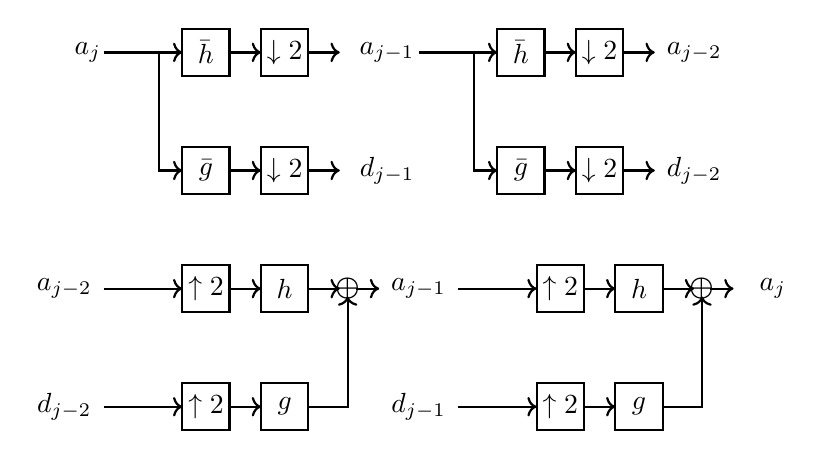
\begin{tikzpicture}[scale=1]
    % Draw the lower picture
    \draw (-0.5,3) node {$a_{j-2}$};
    \draw[->, thick] (0,3) -- (1, 3);
    \draw[thick] (1, 3.3) rectangle (1.6, 2.7);
    \draw (1.3, 3)  node {$\uparrow 2$};
    \draw[thick, ->] (1.6, 3) -- (2,3);
    \draw[thick] (2, 3.3) rectangle (2.6, 2.7);
    \draw (2.3, 3)  node {$h$};
    \draw[thick, ->] (2.6, 3) -- (3,3);
    \draw (3.1, 3) node {$\boldsymbol{\oplus}$};
    
    \draw (-0.5,1.5) node {$d_{j-2}$};
    \draw[->, thick] (0,1.5) -- (1, 1.5);
    \draw[thick] (1, 1.8) rectangle (1.6, 1.2);
    \draw (1.3, 1.5)  node {$\uparrow 2$};
    \draw[thick, ->] (1.6, 1.5) -- (2,1.5);
    \draw[thick] (2, 1.8) rectangle (2.6, 1.2);
    \draw (2.3, 1.5)  node {$g$};
    \draw[thick, ->] (2.6, 1.5) -- (3.1,1.5) -- (3.1, 2.9);
    \draw[thick, ->] (3.2,3) -- (3.5,3);
    \draw (4,3) node {$a_{j-1}$};

    \draw[->, thick] (4.5,3) -- (5.5, 3);
    \draw[thick] (5.5, 3.3) rectangle (6.1, 2.7);
    \draw (5.8, 3)  node {$\uparrow 2$};
    \draw[thick, ->] (6.1, 3) -- (6.5,3);
    \draw[thick] (6.5, 3.3) rectangle (7.1, 2.7);
    \draw (6.8, 3)  node {$h$};
    \draw[thick, ->] (7.1, 3) -- (7.5,3);
    \draw (7.6, 3) node {$\boldsymbol{\oplus}$};
    
    \draw (4,1.5) node {$d_{j-1}$};
    \draw[->, thick] (4.5,1.5) -- (5.5, 1.5);
    \draw[thick] (5.5, 1.8) rectangle (6.1, 1.2);
    \draw (5.8, 1.5)  node {$\uparrow 2$};
    \draw[thick, ->] (6.1, 1.5) -- (6.5,1.5);
    \draw[thick] (6.5, 1.8) rectangle (7.1, 1.2);
    \draw (6.8, 1.5)  node {$g$};
    \draw[thick, ->] (7.1, 1.5) -- (7.6,1.5) -- (7.6, 2.9);
    \draw[thick, ->] (7.7,3) -- (8,3);
    \draw (8.5,3) node {$a_{j}$};
    
    % Draw the upper picture
    \draw (-0.2,6) node {$a_j$};
    \draw[->, thick] (0,6) -- (1, 6);
    \draw[thick] (1, 6.3) rectangle (1.6, 5.7);
    \draw (1.3, 6)  node {$\bar{h}$};
    \draw[thick, ->] (1.6, 6) -- (2,6);
    \draw[thick] (2, 6.3) rectangle (2.6, 5.7);
    \draw (2.3, 6)  node {$\downarrow 2$};
    \draw[thick, ->] (2.6, 6) -- (3,6);
    \draw (3.6,6)  node {$a_{j-1}$};
    
    \draw[thick, ->] (0.7,6) -- (0.7, 4.5) -- (1, 4.5);
    \draw[thick] (1, 4.8) rectangle (1.6, 4.2);
    \draw (1.3, 4.5)  node {$\bar{g}$};
    \draw[thick, ->] (1.6, 4.5) -- (2,4.5);
    \draw[thick] (2, 4.8) rectangle (2.6, 4.2);
    \draw (2.3, 4.5)  node {$\downarrow 2$};
    \draw[thick, ->] (2.6, 4.5) -- (3,4.5);
    \draw (3.6,4.5)  node {$d_{j-1}$};
    
    \draw[->, thick] (4,6) -- (5, 6);
    \draw[thick] (5, 6.3) rectangle (5.6, 5.7);
    \draw (5.3, 6)  node {$\bar{h}$};
    \draw[thick, ->] (5.6, 6) -- (6,6);
    \draw[thick] (6, 6.3) rectangle (6.6, 5.7);
    \draw (6.3, 6)  node {$\downarrow 2$};
    \draw[thick, ->] (6.6, 6) -- (7,6);
    \draw (7.5,6)  node {$a_{j-2}$};
    
    \draw[thick, ->] (4.7,6) -- (4.7, 4.5) -- (5, 4.5);
    \draw[thick] (5, 4.8) rectangle (5.6, 4.2);
    \draw (5.3, 4.5)  node {$\bar{g}$};
    \draw[thick, ->] (5.6, 4.5) -- (6,4.5);
    \draw[thick] (6, 4.8) rectangle (6.6, 4.2);
    \draw (6.3, 4.5)  node {$\downarrow 2$};
    \draw[thick, ->] (6.6, 4.5) -- (7,4.5);
    \draw (7.5,4.5)  node {$d_{j-2}$};
\end{tikzpicture}
\caption{\textbf{Figure 7.12 in S.\ Mallat's book ``\textit{A Wavelet Tour of
Signal Processing}" (3rd edition).} DWT algorithm}

\end{figure}





\begin{figure}

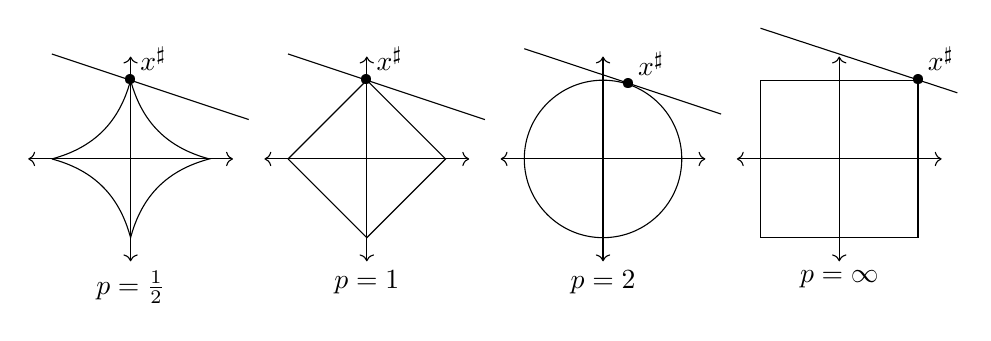
\begin{tikzpicture}

% p = 1/3
\draw[<->] (1.3, 0) -- (-1.3, 0);
\draw[<->] (0, 1.3) -- (0, -1.3) node[below] {$p = \frac{1}{2}$};
\draw[black] (-1,0) 
            to[bend right] (0,1) 
            to[bend right] (1,0) 
            to[bend right] (0,-1) 
            to[bend right] (-1,0);
\draw (-1, 1.333) -- (1.5,0.5);
\draw (0,1) node {\textbullet};
\draw (0,1) node[above right] {$x^{\sharp}$};

% p = 1
\draw[<->] (1.7, 0) -- (4.3, 0);
\draw[<->] (3, 1.3) -- (3, -1.3) node[below] {$p = 1$};
\draw (2,0) -- (3,1) -- (4,0) -- (3, -1) -- (2,0);
\draw (2, 1.333) -- (4.5,0.5);
\draw (3,1) node {\textbullet};
\draw (3,1) node[above right] {$x^{\sharp}$};


% p = 2

\draw[<->] (4.7, 0) -- (7.3, 0);
\draw[<->] (6, 1.3) -- (6, -1.3) node[below] {$p = 2$};
\draw (6,0) circle (1);
\draw (5, 1.4) -- (7.5, 0.57);
\draw (6 + 0.32,0.94) node {\textbullet};
\draw (6 + 0.32,0.94) node[above right] {$x^{\sharp}$};

% p = ∞
\draw[<->] (7.7, 0) -- (10.3, 0);
\draw[<->] (9, 1.3) -- (9, -1.3) node[below] {$p = \infty$};
\draw (8,1) -- (10,1) -- (10,-1) -- (8,-1) -- (8, 1);
\draw(8,1.66) -- (10.5, 0.84);
\draw (10,1) node {\textbullet};
\draw (10,1) node[above right] {$x^{\sharp}$};

\end{tikzpicture}

\caption{(\textbf{Not used in the book}). Norm balls.}
\end{figure}

\begin{figure}
\begin{tikzpicture}[scale=1]
\draw[thick] (0,0) rectangle (5,2);
\draw (0,1) node[left] {$m$};
\draw (2.5,2) node[above] {$N$};
\draw[thick] (5.2,-1.5) rectangle (5.7,3.5); 
\draw[thick] (6.5,0) rectangle (7.0,2); 
\draw (6.1,1) node {$=$};

\draw (5.45,1) node[cross] {};
\draw (5.45,3.35) node[cross] {};
\draw (5.45,3.1) node[cross] {};
\draw (5.45,1.7) node[cross] {};
\draw (5.45,-1.0) node[cross] {};

\draw (3.5,-1.9)  node {$Ax = b$};
%\draw (5.45,-1.9) node {$\x$};
%\draw (6.75,-1.9) node {$\b$};
%\draw (6.1,-1.9) node {$=$};

\end{tikzpicture}
\caption{(\textbf{Not used in the book}). Underdetermined linear system where $x$ is sparse.}
\end{figure}










\begin{figure}



\end{figure}












\end{document}

